\documentclass[]{article}

% to define bibliography and insert cites
\usepackage[backend=biber]{biblatex}
\addbibresource{references.bib}

% multilanguage
\usepackage[english,spanish]{babel} 

\newenvironment{poliabstract}[1]
	{\renewcommand{\abstractname}{#1}\begin{abstract}}
	{\end{abstract}}

% to insert fragments of code
\usepackage{listings}

% to make links clickable
\usepackage{hyperref}
\hypersetup{colorlinks=false,linktoc=all}

% include images
\usepackage{graphicx}
\usepackage{caption}    % contains subpackage 'subcaption'
\usepackage{subcaption} % allows subfigures
\usepackage{float}      % allows floating H to place images in certain place

% paragraph spacing
\usepackage{parskip}
\usepackage{setspace}

% avoid numbering in equation
\usepackage{amsmath}

% coloring text
\usepackage{xcolor}

% beautiful tables
\usepackage{booktabs}

% caption font
\usepackage{caption}
\captionsetup[figure]{font=small, labelfont=bf}
\captionsetup[table]{font=small, labelfont=bf}

% language redefinitions
\addto\captionsspanish{%
	\renewcommand*\contentsname{Contenido}
	\renewcommand{\figurename}{Figura}
	\renewcommand{\tablename}{Tabla}
}

\begin{document}

\begin{titlepage}
	\centering
	
\includegraphics[width=0.5\textwidth]{images/logo_utad.jpg}\par\vspace{1cm}
	{\large\bfseries Sistema de detección automática de baches en el asfalto a partir de imágenes\par}
	\vspace{1.5cm}
	{\large \itshape Diego Castro Viadero\par}
	Septiembre 2019\par
	\vspace{1.5cm}
	{\small Tutor: Ricardo Moya García}
\end{titlepage}

\selectlanguage{spanish}
\begin{poliabstract}{Resumen}
\noindent
El estado del asfalto en carreteras tanto de ámbito nacional como de ámbito urbano es de alta importancia en relación a la seguridad vial. En la actualidad, gracias a los avances tecnológicos, se están desarrollando sistemas de detección automática de baches en el asfalto, permitiendo una detección precoz de estas irregularidades en la carretera.

\doublespacing\singlespacing
\noindent
Este proyecto pretende contribuir en este ámbito desarrollando un sistema de detección automática de baches a partir de imágenes. Partiendo de un conjunto de imágenes etiquetadas con baches, se ha entrenado una red neuronal \textit{YOLO V3} y otra \textit{YOLO V3 Tiny}. El entrenamiento se ha realizado con distintos tamaños de red y con distintos subconjuntos de imágenes, dando lugar a un total de quince modelos. Tras un estudio comparativo de las precisiones de los modelos, aquellos con mejores resultados han sido exportados y transformados para ser ejecutables en un dispositivo móvil. Finalmente se ha desarrollado una aplicación móvil Android que carga los modelos anteriormente exportados y los ejecuta utilizando como entrada la salida de la cámara del dispositivo.
\end{poliabstract}

\selectlanguage{english}
\begin{poliabstract}{Abstract}
\noindent
The state of asphalt on both national and urban roads is of high importance in relation to road safety. Currently, thanks to technological advances, automatic detection systems are being developed to detect potholes in the asphalt, allowing early detection of these irregularities on the road.

\doublespacing\singlespacing
\noindent
This project aims to contribute to this field by developing an automatic pothole detection system based on images. Starting from a set of images labeled with potholes, a neural network YOLO v3 and another YOLO v3 Tiny have been trained. The training has been carried out with different network sizes and with different subsets of images, resulting in fifteen models. After a comparative study of the precisions of the models, those with better results have been exported and transformed to be executable in a mobile device. Finally, an Android mobile application has been developed that loads the previously exported models and executes them using the camera output of the device as input.
\end{poliabstract}

\newpage
\begin{flushright}
	\section*{Agradecimientos}
	 A mi tutor Ricardo Moya García, por su esfuerzo, dedicación, consejo y por guiarme y darme ánimos en todo momento.
	 
	 A mi pareja Nerea, por toda la paciencia que ha tenido y por el apoyo que me ha brindado a lo largo de esta aventura.
\end{flushright}

\newpage
\selectlanguage{spanish}
\tableofcontents{}

\newpage
\section{Introducción}

\subsection{Motivación y Objetivos}

En los últimos años las prioridades en relación a la seguridad vial han provocado un cambio de mentalidad en la sociedad.  Muchos de los últimos avances tecnológicos están orientados al desarrollo de medios de transporte más seguros. Uno de estos avances que contribuye a la mejora de la seguridad es la inclusión de un sistema de detección de desperfectos en la calzada.

%cambio mentalidad, priorizacion de la seguridad vial
%avances tecnológicos en medios de transporte orientados a la mejora de la seguridad vial
%un area de mejora en la se ha invertido es en la inclusión de sistemas de detección de irregularidades en el asfalto en los vehiculos

En la actualidad, en el ayuntamiento de Madrid, existe un sistema de sugerencias y reclamaciones \cite{s1_syr} que permite al ciudadano, entre otras opciones, denunciar la existencia de irregularidades en el asfalto, tener un registro de las mismas y planificar su subsanación. Según el informe de sugerencias y reclamaciones del ayuntamiento de Madrid \cite{s1_syrreport}, en el primer semestre del año, se registraron 3.000 reclamaciones en materia de \textit{vías y espacios públicos} de las cuales el 50\% correspondieron a la submateria \textit{aceras y calzadas}.

Este sistema de funcionamiento actual, que delega en el ciudadano la tarea de reporte de este tipo de desperfectos, dificulta y retrasa la puesta en conocimiento de las irregularidades a las autoridades responsables aumentando la probabilidad de que suceda algún incidente.

Algunas marcas de vehículos han desarrollado innovaciones, que son capaces de detectar baches cuando pasan sobre ellos y adaptar la dureza de la suspensión para conseguir una conducción más segura y cómoda. También contemplan un envío sistemático de la detección de baches, en tiempo real, tanto a otros vehículos como a las autoridades pertinentes. Otras marcas plantean la inclusión de cámaras que permitan la detección del bache sin necesidad de pasar por encima de este.

Con estas innovaciones se recupera el control sobre la detección de baches, liberando al ciudadano de esta tarea y reduciendo la probabilidad de incidentes gracias a disponer de la información con más antelación.

Este trabajo trata de desarrollar un sistema de detección de baches en tiempo real en línea con los últimos avances tecnológicos. El objetivo es entrenar una red neuronal con un conjunto de imágenes donde los baches han sido etiquetados previamente y obtener como resultado un modelo exportable para ser ejecutado en un dispositivo móvil.

Gracias a este trabajo he podido ampliar los conocimientos adquiridos durante el máster de Big Data \& Data Science, impartido por la U-TAD, centrando el proyecto en el procesamiento de imágenes y tratando al mimso tiempo que tenga una utilidad social.

% (porque has hecho este proyecto y que objetivos persigues)
% motivación: aplicar los conocimientos adquiridos durante el master en un proyecto "real"
% adquirir/complementar conocimientos que faltan en el máster

\subsection{Estructura del trabajo}

% (este punto es pura formalidad. Se suele poner uno o dos párrafos explicando la estructura del proyecto como hacen en los libros)
% en el tema X se hablará de tatata, en el tema Y se hablará de blablabla

{\color{red} \textbf{!!! TODO}} % (2-4 páginas)

\newpage
\section{Estado del arte}

% En el punto de motivación y objetivos debes de dejar muy claro que es lo que quieres hacer (un detector de baches) y en este tema 2 debes de explicar como se solucionan este tipo de problemas (CNN) y las redes y frameworks existentes para poder realizar tu trabajo. Como esto ya es una cosa que has hecho (me lo mandaste en un mail muy bien explicado) debes de contar los pros y contras y justificar el porque has seleccionado la red seleccionada

El problema que se pretende resolver podría ser afrontado de dos posibles maneras:

\begin{itemize}
	\item Como un problema de clasificación de imágenes
	\item Como un problema de detección de objetos
\end{itemize}

El primero de los enfoques es más sencillo y está más estudiado. Dada una imagen, se determina una clase a la que pertenece la imagen. En los problemas de clasificación cada una de las imágenes se centran en un único objeto. Este tipo de problemas de clasificación se resuelven comúnmente con redes neuronales convolucionales. Existen numerosas arquitecturas de redes neuronales convolucionales ya definidas y estudiadas para resolver este tipo de problemas, como por ejemplo: VGG-16, LeNet, ResNet, GoogLeNet/Inception, etc.

El segundo de los enfoques es más complicado, y presenta varios retos. El primero de ellos es que las imágenes no se centran en un único objeto, sino que puede haber múltiples objetos a detectar y además tratarse de objetos de distintos tipos. El segundo de los restos es el tamaño de los objetos a identificar, que puede ser variable. Y el tercero de los retos es que se están resolviendo dos problemas al mismo tiempo: localizar objetos en una imagen y clasificar los objetos localizados.

Para resolver los problemas de detección de objetos existen dos aproximaciones. La primera de las aproximaciones es una aproximación clásica, basada en técnicas de machine learning. Un ejemplo representativo de esta aproximación clásica es Viola-Jones, que se basa en clasificadores binarios y que se ha usado en las cámaras de fotos para la detección de caras.

El uso del deep learning para la detección de objetos ha supuesto una revolución y ha cambiado las reglas del juego. Esta aproximación para la resolución de este tipo de problemas es relativamente reciente y ha estado en constante evolución.

{\color{red} \textbf{!!! TODO}}

\begin{itemize}
	\item R-CNN
	\item Fast R-CNN
	\item Faster R-CNN
	\item SDD
	\item YOLO (YOLO, YOLOv2, YOLOv3)
	\item Mask R-CNN
\end{itemize} % (como mucho 10 páginas)

\newpage
\section{Definición de requisitos y análisis}
\label{sec:definicion_de_requisitos_y_analisis}

\subsection{Definición de requisitos}

A continuación se enumeran los requisitos para el desarrollo del trabajo:

\begin{itemize}
	\item Implementar y entrenar una red neuronal que genere un modelo capaz de detectar baches en el asfalto a partir de imágenes
	\item El modelo deberá ser capaz de procesar una imagen en un tiempo lo más cercano posible a 1/30s, para ser capaz de procesar video en tiempo real
	\item El modelo deberá poderse ejecutar en un dispositivo móvil Android
	\item El modelo será alimentado directamente con la salida de la cámara del dispositivo móvil
\end{itemize}

\subsection{Arquitectura}

\begin{figure}[H]
	\centering
	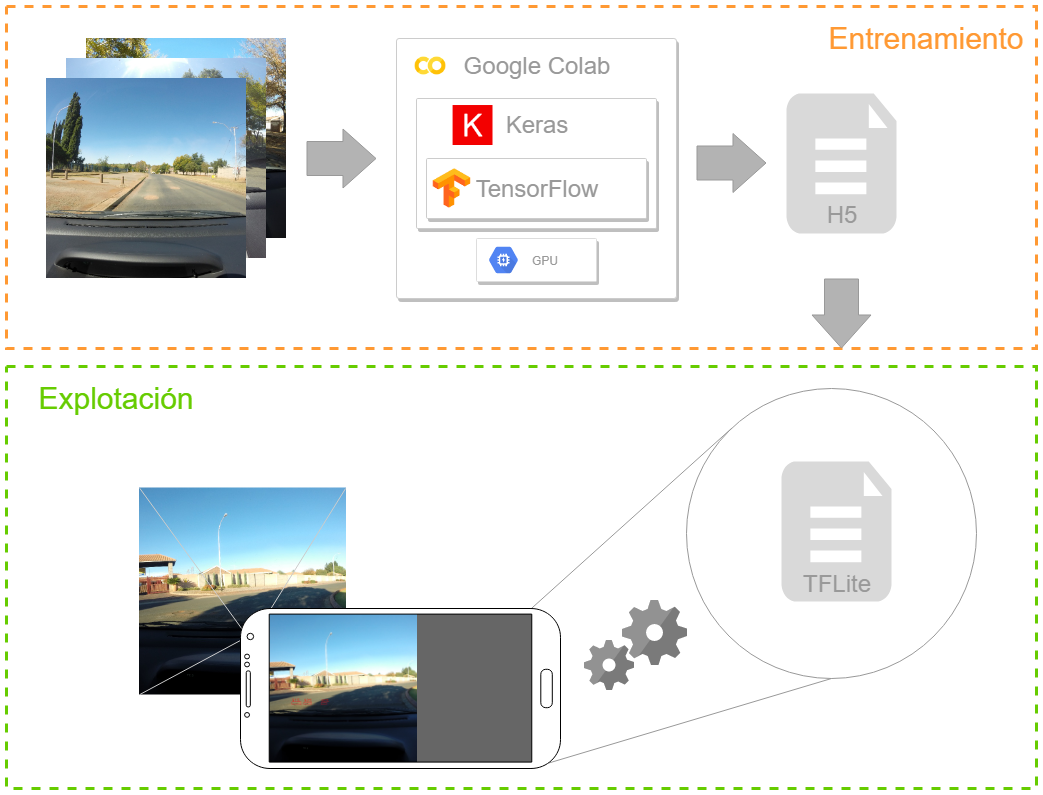
\includegraphics[width=\linewidth]{images/architecture.png}
	\caption{Arquitectura}
	\label{fig:architecture}
\end{figure}

Como se puede observar en la figura \ref{fig:architecture}, la arquitectura está dividida en dos partes. Una parte se utiliza para entrenar la red neuronal y generar el modelo. La otra parte se utiliza para explotar el modelo generado.

El entrenamiento de la red neuronal requiere de una infraestructura con un hardware potente, que incluya GPU para reducir los tiempos de entrenamiento. Sin embargo la explotación del modelo generado, no  requiere de un hardware potente, y puede ejecutarse directamente en un dispositivo móvil en posesión del usuario final. El modelo obtenido después de la fase de entrenamiento requiere de una transformación a un formato concebido para ser ejecutado en dispositivos con recursos limitados.

\subsection{Tecnologías}

Todo el proyecto ha sido desarrollado utilizando Python, a excepción de la aplicación Android, que ha sido desarrollada en Java.

Para todo lo relacionado con el tratamiento de imágenes se ha utilizado el paquete de python OpenCV. Este tratamiento incluye la lectura de imágenes, recorte, reescalado y volteo de las imágenes, visualización de las predicciones obtenidas, etc.

Para la implementación de la red neuronal se ha utilizado Keras, que es un envoltorio sobre Tensorflow que simplifica su uso. Dada una arquitectura de red neuronal, con Keras es muy sencillo definir las capas y sus interconexiones. Además Keras proporciona clases que facilitan la definición de un conjunto de imágenes como entrada de la red neuronal. Keras también proporciona una serie de eventos con la idea de poder suscribirse a los mismos y poder reaccionar en consecuencia, como por ejemplo, suscribirse al evento de final de época y salvar el modelo si este ha mejorado con respecto a la época anterior.

Después de realizar un estudio del estado del arte en la resolución de problemas de detección de objetos y con los requisitos definidos para el proyecto, se ha decidido optar por la utilización de YOLO para el desarrollo del mismo. Concretamente se van a utilizar dos versiones de YOLO: \textit{YOLO V3 Tiny}, diseñada para ejecutarse en dispositivos con recursos limitados y \textit{YOLO V3}, para compararla con la anterior. El proyecto se basa en un par de implementaciones de YOLO para Keras \footnote{https://github.com/experiencor/keras-yolo3} \footnote{https://github.com/HoracceFeng/keras-yolo3-tiny}. Se han unido ambas implementaciones en una única \footnote{https://github.com/dicastro/tfm/tree/tfm-yolo3-tiny} que soporta ambas versiones de YOLO. Además, se han realizado múltiples desarrollos complementarios para mejorar la funcionalidad, como por ejemplo, adición de soporte en formato txt para el etiquetado de las imágenes y adición de nuevos parámetros de configuración para mejorar el resultado del entrenamiento.

Para la ejecución de los modelos obtenidos en un dispositivo móvil de ha utilizado TFLite. Este paquete permite transformar distintos tipos de modelo (keras, tensorflow) a formato TFLite y ejecutar estos modelos en dispositivos con recursos reducidos. En las últimas versiones de esta librería se soporta, aunque de forma experimental, el uso de la GPU del dispositivo.

La aplicación móvil ha sido desarrollada en java para la plataforma Android. Se ha hecho uso de la librería de TFLite, disponible para java, que hace que la carga y ejecución del modelo sea una tarea trivial. % (2-4 páginas)

\newpage
\section{Datos}

\subsection{Descripción de las fuentes de datos a utilizar}

El juego de datos ha sido obtenido de kaggle \cite{s4_potholedataset} y se compone de un total de 1900 imágenes, tomadas desde el interior de un coche, con un tamaño igual a 3680x2760 píxeles (formato 4:3), y de un conjunto de ficheros de texto con el etiquetado de las mismas. Las imágenes se dividen en dos subconjuntos: uno de 1297 imágenes para el entrenamiento y otro de 603 imágenes para la evaluación del modelo. Por cada uno de los subconjuntos de imágenes existe un fichero de texto con el etiquetado de las mismas. Cada una de las líneas del los ficheros de texto contiene las etiquetas de una imagen. La estructura de cada línea es la siguiente:

\begin{lstlisting}[frame=single,basicstyle=\ttfamily\footnotesize]
<RUTA_IMG> <NUMERO_DE_ETIQUETAS>( <X0> <Y0> <ANCHO> <ALTO>)+
\end{lstlisting}

Para facilitar el posterior tratamiento, se ha realizado una transformación del formato de los ficheros de etiquetas al siguiente formato:

\begin{lstlisting}[frame=single,basicstyle=\ttfamily\footnotesize]
<RUTA_IMG>( <X0>,<Y0>,<ANCHO>,<ALTO>,<CLASE>)+
\end{lstlisting}

\subsection{Estudio de los datos}

En una fase inicial se ha realizado un análisis del tamaño de los socavones con respecto al tamaño de la imagen. Esto es un aspecto importante a tener en cuenta de cara a determinar el algoritmo a utilizar para la detección de objetos. Los algoritmos de detección de objetos, en general se comportan peor cuanto más pequeños son los objetos a detectar.

Como se observa en la figura \ref{fig:potholesizes}, la mayoría de los socavones tienen una anchura inferior a 200 píxeles y una altura inferior a 50 píxeles. Este factor será tenido en cuenta en el preprocesamiento de las imágenes.

\begin{figure}[H]
	\centering
	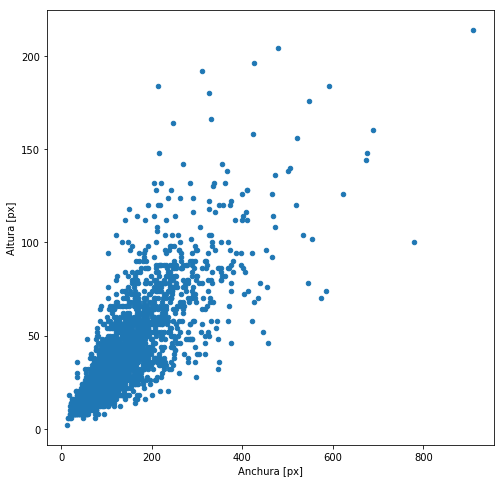
\includegraphics[width=0.7\linewidth]{images/pothole_sizes_scatter_plot.png}
	\caption{Tamaños de los socavones en píxeles}
	\label{fig:potholesizes}
\end{figure}

También se ha realizado un estudio de la localización de los socavones en las imágenes. Tal y como se ve en la figura \ref{fig:potholeslocations}, los baches están localizados principalmente en el centro de la imagen. La parte inferior se corresponde con el salpicadero del coche y la parte superior se corresponde con paisaje.

\begin{figure}[H]
	\centering
	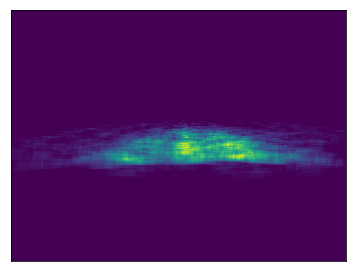
\includegraphics[width=0.7\linewidth]{images/pothole_locations_heatmap.png}
	\caption{Localizaciones de los socavones en las imágenes}
	\label{fig:potholeslocations}
\end{figure}

\subsection{Preprocesamiento de las imágenes}
\label{subsec:preprocesamiento_de_las_imagenes}

Tanto en la fase de entrenamiento, como para hacer una predicción, las imágenes van a ser redimensionadas al tamaño de la red neuronal, la cual tiene una relación de aspecto 1:1. Para redimensionar una imagen con una relación de aspecto 4:3, y al mismo tiempo, transformarla en una imagen con relación de aspecto 1:1, lo que se hace es redimensionar el lado más grande de la imagen manteniendo la relación de aspecto, es decir, aplicando el mismo factor de redimensionamiento al lado más pequeño. Una vez redimensionada, se rellena con gris la zona superior y la zona inferior de la imagen para cuadrarla. En la figura \ref{fig:imagedirectresize} se muestra un ejemplo gráfico.

\begin{figure}[H]
	\centering
	\begin{subfigure}[h]{0.45\linewidth}
		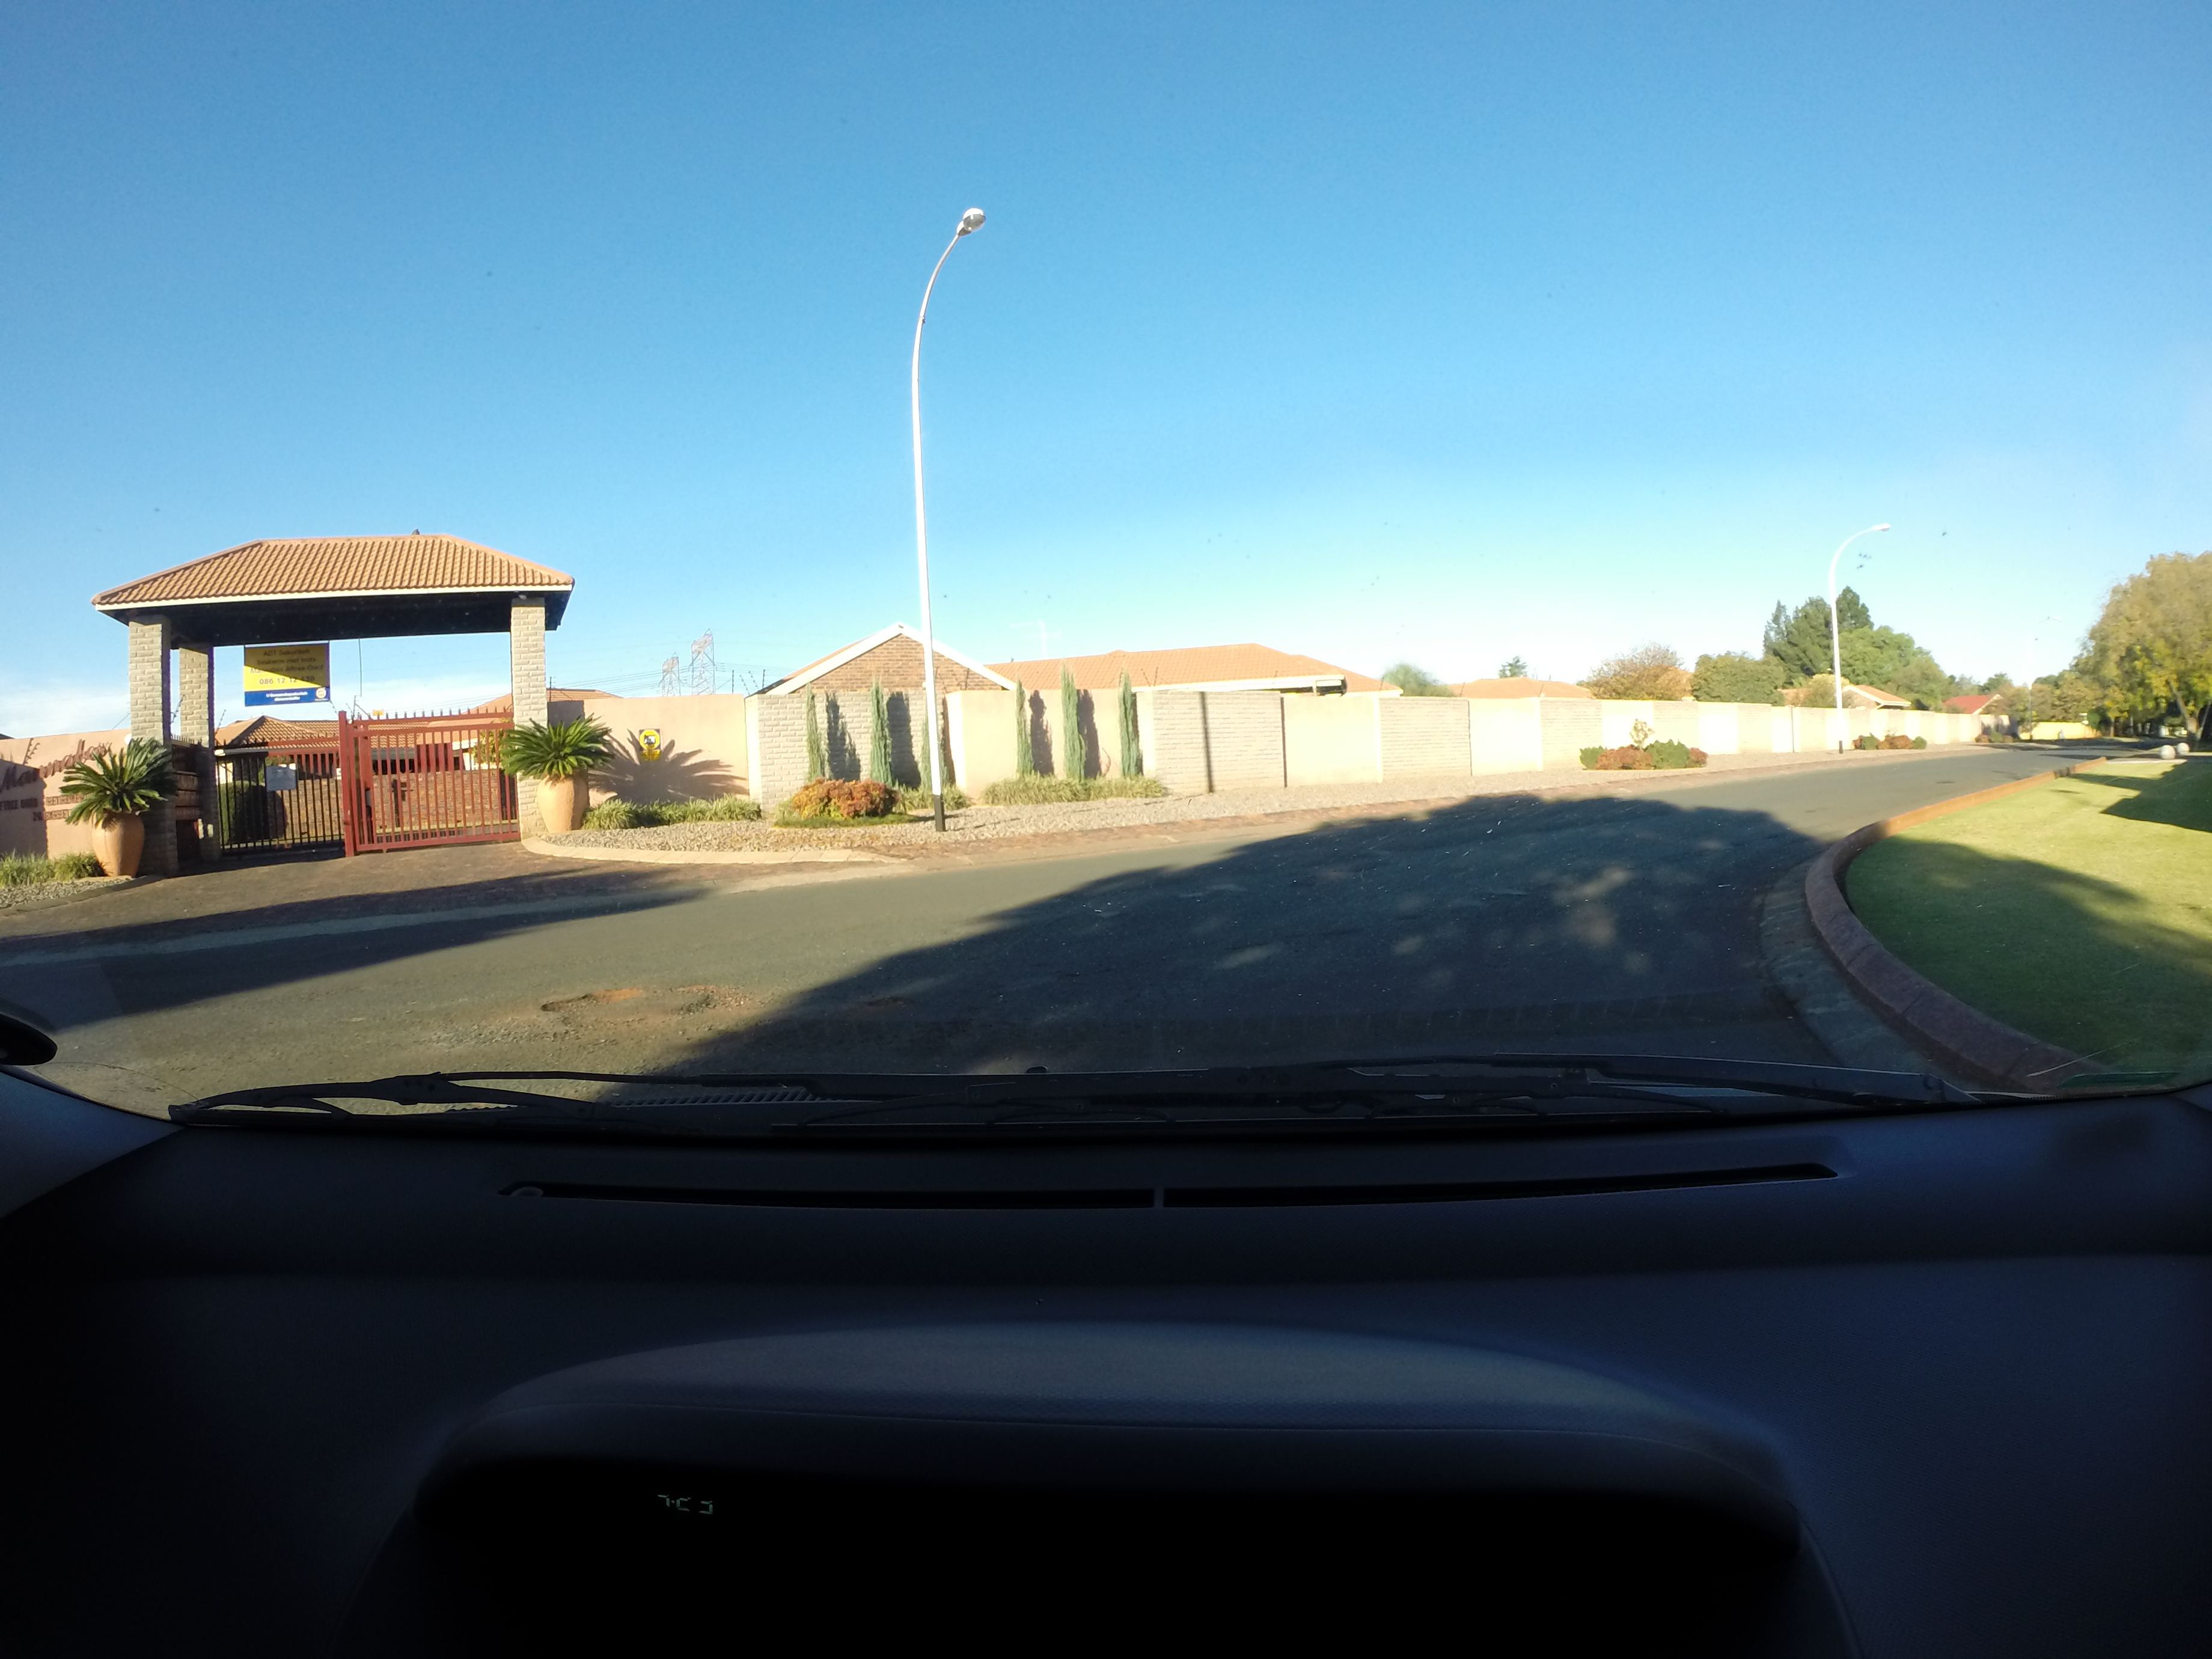
\includegraphics[width=\linewidth]{images/image_direct_resize_before.jpg}
	\end{subfigure}
	\begin{subfigure}[h]{0.45\linewidth}
		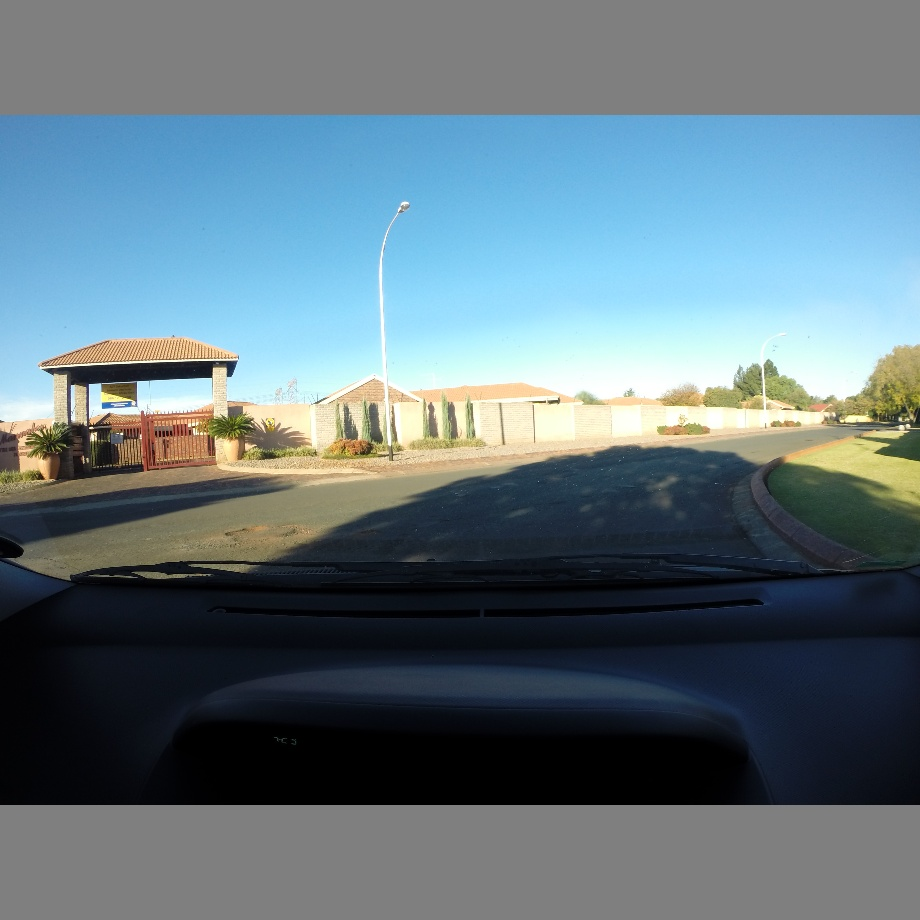
\includegraphics[width=\linewidth]{images/image_direct_resize_after.jpg}
	\end{subfigure}
	\caption{A la izquierda la imagen original redimensionada a tamaño 920x690 px (manteniendo la relación de aspecto 4:3). A la derecha la imagen redimensionada con el relleno para que tenga una relación de aspecto 1:1 (920x920 px)}
	\label{fig:imagedirectresize}
\end{figure}

El redimensionamiento se hace en base al lado más grande de la imagen, que en el ejemplo anterior es la anchura. Para determinar el factor de redimensionamiento, se divide la anchura la imagen final entre la anchura de la imagen original, en este caso: $920 / 3680 = 0.25$. A continuación, se aplica este factor de redimensionamiento a ambos lados de la imagen, resultando en un tamaño de 920x690 píxeles. Por último se calcula el relleno que haría falta a cada lado de la imagen: $(920 - 690) / 2 = 115$.

Siguiendo con este ejemplo, si en la imagen original hubiese un socavón de tamaño 160x24 píxeles, y se aplicase este factor de redimensionamiento, el socavón redimensionado tendría unas dimensiones de 40x6 píxeles, lo cual sería un tamaño bastante pequeño ya que únicamente tiene 6 píxeles de alto (de 920 que tiene la imagen).

Sin embargo, si previo al redimensionamiento de la imagen, se recortan los extremos izquierdo y derecho de la imagen, de tal forma que tenga una relación de aspecto 1:1, se consigue que el factor de redimensionamiento sea mayor y que por tanto los socavones redimensionados sean también más grandes. Esta técnica tiene un inconveniente, y es que la imagen original se está recortando, por lo que está habiendo una pérdida de información. Este inconveniente no es un impedimento, ya que en el apartado ~\ref{subsec:preprocesamiento_de_las_imagenes} se ha comprobado que la mayor parte de los socavones están en el centro de las imágenes, y que recortando los extremos de las mismas la pérdida de información es mínima.

Para aplicar esta técnica, en primer lugar habría que calcular los recortes que hay que hacer a cada lado de la imagen original. Para ello se calcula la diferencia entre la anchura y la altura de la imagen y se divide por dos: $(3680 - 2760) / 2 = 460$. Una vez recortada la imagen se calcula el factor de redimensionamiento: $920 / 2760 = 0.333$. Por último se aplicaría este factor de redimensionamiento a la altura y la anchura de la imagen.

Si aplicamos este nuevo factor de redimensionamiento al tamaño del socavón del ejemplo anterior (160x24 píxeles), el tamaño del socavón redimensionado sería 53x8 (un 75\% más grande). % (<4 páginas)

\newpage
\section{Técnicas de Deep Learning y métodos de evaluación}
\label{sec:tecnicas_de_deep_learning_y_metodos_de_evaluacion}

\subsection{Técnicas de Deep Learning a utilizar en el proyecto}

A continuación se explicarán las principales técnicas utilizadas para el desarrollo del proyecto. Algunas de las técnicas que se mencionan no son específicas del deep learning.

\subsubsection*{\textit{Hold-out}}

El entrenamiento de las redes neuronales YOLO se ha realizado siguiendo esta técnica. Hold-out no es una técnica específica del deep learning, sino que es una técnica general que aplica sobre cualquier algoritmo de aprendizaje. Consiste en dividir el conjunto de datos en dos subconjuntos: uno que se utiliza para el entrenamiento y otro que únicamente se utiliza para evaluar el modelo obtenido tras el entrenamiento.

\subsubsection*{\textit{Red Neuronal Convolucional (CNN)}}

Tal y como se ha comentado en el apartado \textit{\nameref{sec:estado_del_arte}}, YOLO es una red neuronal convolucional, por lo que antes de entrar en los detalles se va a explicar cómo funciona una CNN \cite{s5_cnn1} \cite{s5_cnn2}.

Las CNNs están compuestas por una sucesión de capas convolucionales, para la extracción de características, seguidas de unas capas perceptrón simples, para la clasificación final. Las capas convolucionales forman una jerarquía, de forma que las capas del principio son capaces de detectar formas básicas y cuanto más ``profunda'' es la capa, más complejas son las formas que son capaces de detectar. Por ejemplo: una capa inicial sería capaz de detectar líneas y círculos, mientras que una capa profunda sería capaz de detectar una cara.

Cada capa convolucional recibe como entrada una matriz bidimensional. En el caso de tratarse de la primera capa la entrada se corresponde directamente con la imagen, si se trata de una capa más profunda la entrada se corresponde con la salida de la capa anterior. Además, cada capa tiene definido un \textit{kernel}, que no es más que otra matriz bidimensional de dimensiones reducidas. Con la matriz de entrada y el kernel se realiza la operación de \textit{convolución}.

\begin{figure}[H]
	\centering
	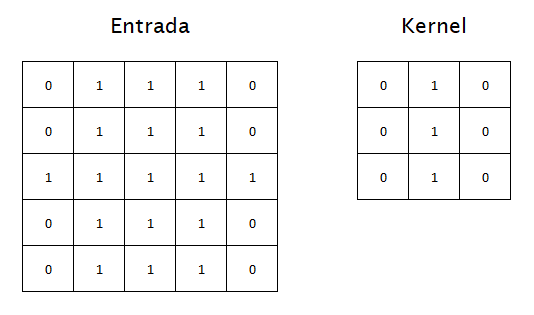
\includegraphics[width=0.7\linewidth]{images/convolutional_neuron_example.png}
	\caption{Ejemplo de capa convolucional con una entrada de 5x5 y un kernel de 3x3}
	\label{fig:cnn_neuronex}
\end{figure}

La operación de \textit{convolución} consiste en hacer un barrido del \textit{kernel} por la matriz de entrada, de izquierda a derecha y de arriba a abajo. En cada una de las posiciones del barrido se aplica el producto escalar entre el kernel y la submatriz de la matriz de entrada sobre la que se encuentre. En la figura \ref{fig:cnn_convolutionoperationex} se puede ver gráficamente el proceso.

\begin{figure}[H]
	\centering
	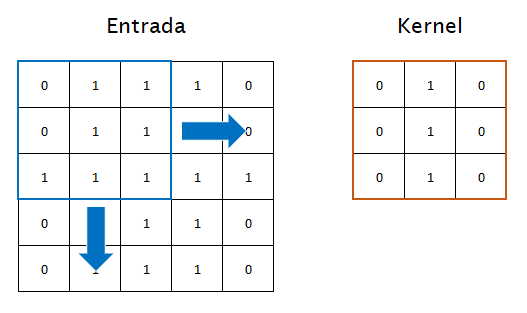
\includegraphics[width=0.7\linewidth]{images/convolutional_operation_example.png}
	\caption{Representación gráfica de operación convolucional}
	\label{fig:cnn_convolutionoperationex}
\end{figure}

Para realizar el producto escalar, las matrices se \textit{aplanan}, de tal forma que la submatriz de entrada quedaría de la siguiente forma:

\begin{equation}
	\left[
	\begin{array}{ccc}
		0 & 1 & 1 \\
		0 & 1 & 1 \\
		0 & 1 & 1 \\
	\end{array}
	\right]
	=>
	\left[
	\begin{array}{ccccccccc}
		0 & 1 & 1 & 0 & 1 & 1 & 0 & 1 & 1 \\
	\end{array}
	\right]
	\nonumber
\end{equation}

El kernel:

\begin{equation}
	\left[
	\begin{array}{ccc}
		0 & 1 & 0 \\
		0 & 1 & 0 \\
		0 & 1 & 0 \\
	\end{array}
	\right]
	=>
	\left[
	\begin{array}{ccccccccc}
		0 & 1 & 0 & 0 & 1 & 0 & 0 & 1 & 0 \\
	\end{array}
	\right]
	\nonumber
\end{equation}

Y por lo tanto el producto escalar:

\begin{equation}
	\left[
	\begin{array}{ccccccccc}
		0 & 1 & 1 & 0 & 1 & 1 & 0 & 1 & 1 \\
	\end{array}
	\right]
	\left[
	\begin{array}{c}
		0 \\
		1 \\
		0 \\
		0 \\
		1 \\
		0 \\
		0 \\
		1 \\
		0 \\
	\end{array}
	\right] = 3
	\nonumber
\end{equation}

Como resultado de aplicar la convolución sobre la matriz de entrada se obtiene una nueva matriz. Además del kernel, las capas convolucionales tienen otros parámetros asociados, como por ejemplo, cómo de rápido avanza el kernel durante el barrido.

Las capas convolucionales no tiene un único kernel asociado, sino que tienen varios. Teniendo en cuenta esto y suponiendo que tenemos como entrada una imagen en blanco y negro de $28x28x1$ píxeles y que cada capa tiene $32$ kernels de $3x3$, la primera capa convolucional estaría compuesta por $28 x 28 = 784$ neuronas, y tras aplicar la operación de convolución, se obtendrían como resultado $32$ nuevas matrices de dimensiones $26 x 26$, que harían necesarias $26 x 26 x 32 = 21.632$ neuronas en la segunda capa. Teniendo en cuenta que una CNN puede estar compuesta por varias decenas de capas, se hace necesario introducir un mecanismo de reducción, para que el número de neuronas necesarias no crezca tan desmesuradamente con cada capa. Este mecanismo se conoce como \textit{pooling}. El \textit{MaxPooling}, es un tipo de pooling comunmente usado, y consiste en deslizar una ventana bidimensional sobre la matriz de entrada, de izquierda a derecha y de arriba a abajo. En cada una de las posiciones se tomará como valor resultante el máximo valor presente en la ventana. La capacidad de reducción del MaxPooling depende de dos factores: el tamaño de la ventana y el tamaño del salto que se da hacia la derecha y hacia abajo. En la figura \ref{fig:cnn_maxpooling} se muestra un ejemplo gráfico.

\begin{figure}[H]
	\centering
	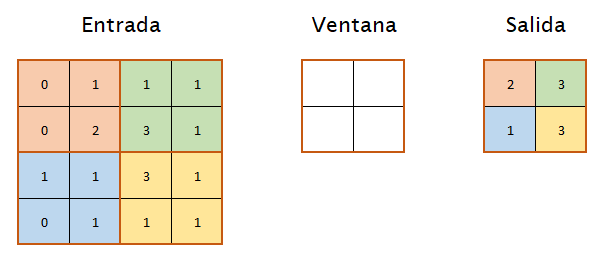
\includegraphics[width=0.7\linewidth]{images/maxpooling_example.png}
	\caption{Representación gráfica de MaxPooling con una entrada de 4x4, una ventana de 2x2 y un salto de 2}
	\label{fig:cnn_maxpooling}
\end{figure}

\subsubsection*{Transferencia de conocimiento (transfer learning)}

% Otra de las técnicas que se han utilizado en el proyecto es la denominada \textit{transferencia del conocimiento (transfer learning)}.

Entrenar un modelo de detección de objetos es un proceso muy costoso, ya que se necesita un gran volumen de imágenes y una gran capacidad de cómputo. El \textit{transfer learning} viene a paliar este problema ya que permite utilizar un modelo ya entrenado como punto de partida para entrenar otro. Como se ha comentado anteriormente, las primeras capas de una CNN son capaces de detectar formas básicas y a medida que se profundiza en las capas, estas detectan formas más específicas. Si ya tenemos entrenado un modelo \texttt{X} para detectar un determinado tipo de objetos y queremos entrenar otro \texttt{Y} para detectar otro tipo de objetos, las primeras capas de ambos modelos van a detectar el mismo tipo de formas, y serán las capas más profundas las que se diferencien. Por lo tanto podríamos utilizar el modelo \texttt{X} como punto de partida para el modelo \texttt{Y}, y este último podrá beneficiarse del conocimiento transferido aprender más rápido.

Esta técnica se ha utilizado ampliamente durante la fase de entrenamiento. Se ha utilizado para aprovechar el conocimiento de los modelos YOLO ya entrenados proporcionados por sus autores. También se ha utilizado para lidiar con las limitaciones de uso que tiene la infraestructura utilizada durante el entrenamiento.

\subsubsection*{YOLO V3}

En la figura \ref{fig:yolov3architecture} se muestra la arquitectura de YOLO V3 de tamaño 416x416. Está compuesta por un total de 106 capas convolucionales. Tiene una única entrada, de dimensiones 416x416x3, y tres salidas de dimensiones 13x13x255, 26x26x255 y 52x52x255 respectivamente. Las tres salidas se corresponden con 3 escalas de detección de objetos, la primera de ellas sirve para detectar objetos grandes, la segunda objetos medianos y la tercera objetos pequeños.

Como se explicó en la sección \textit{\nameref{sec:estado_del_arte}}, YOLO divide la imagen en una rejilla de $SxS$ celdas. En realidad, divide la imagen en tres rejillas que se corresponden con las 3 salidas. Para cada una de las celdas de estas rejillas se proponen un número $B$ regiones candidatas, en este caso son 5. Cada una de estas regiones candidatas están representadas por 5 variables, 4 para la región propiamente dicha y 1 para indicar la probabilidad de que la región contenga un objeto. YOLO es capaz de detectar 80 clases de objetos, por lo que junto a cada región candidata se añaden otras 80 variables para indicar la probabilidad de pertenencia a cada una de las clases. Con todo esto, cada una de las celdas de las rejillas se compone de $3 x (5 + 80) = 255$ variables.

\begin{figure}[H]
	\centering
	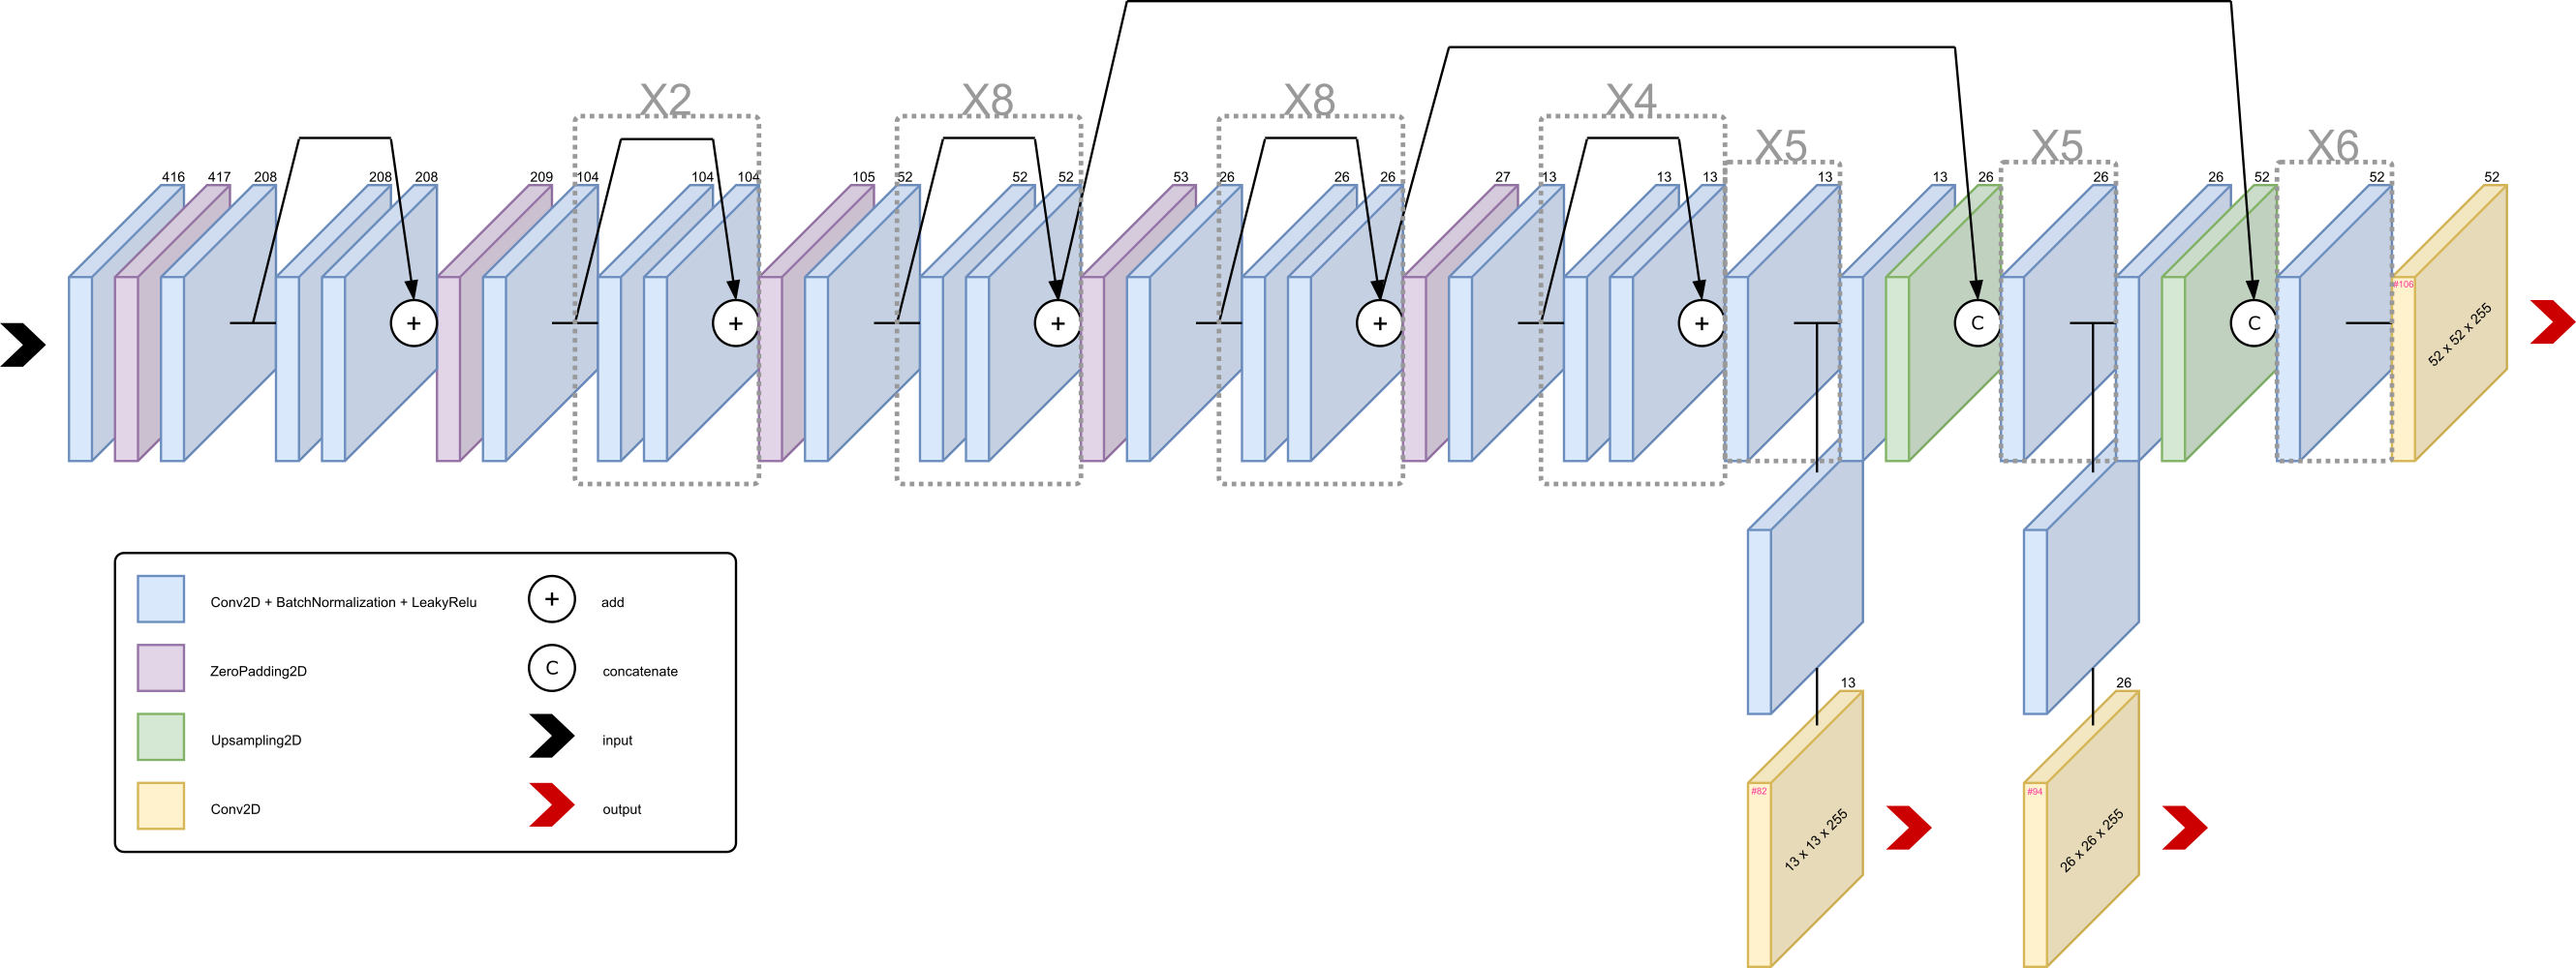
\includegraphics[width=\linewidth]{images/yolo_v3_architecture.png}
	\caption{Arquitectura de YOLO V3 de tamaño 416x416}
	\label{fig:yolov3architecture}
\end{figure}

\subsubsection*{YOLO V3 Tiny}

En la figura \ref{fig:yolov3tinyarchitecture} se muestra la arquitectura YOLO V3 Tiny de tamaño 416x416. Está compuesta por un total de 13 capas convolucionales. Tiene una única entrada, de dimensiones 416x416, y dos salidas de dimensiones 13x13x255 y 26x26x255 respectivamente. El fundamento es el mismo que en YOLO V3. Se han reducido el número de capas convolucionales de manera considerable, lo cual simplifica el modelo y hace que sea apto para ejecutarse en un dispositivo con recursos limitados manteniendo la premisa de ser capaz de detectar objetos en tiempo real.

\begin{figure}[H]
	\centering
	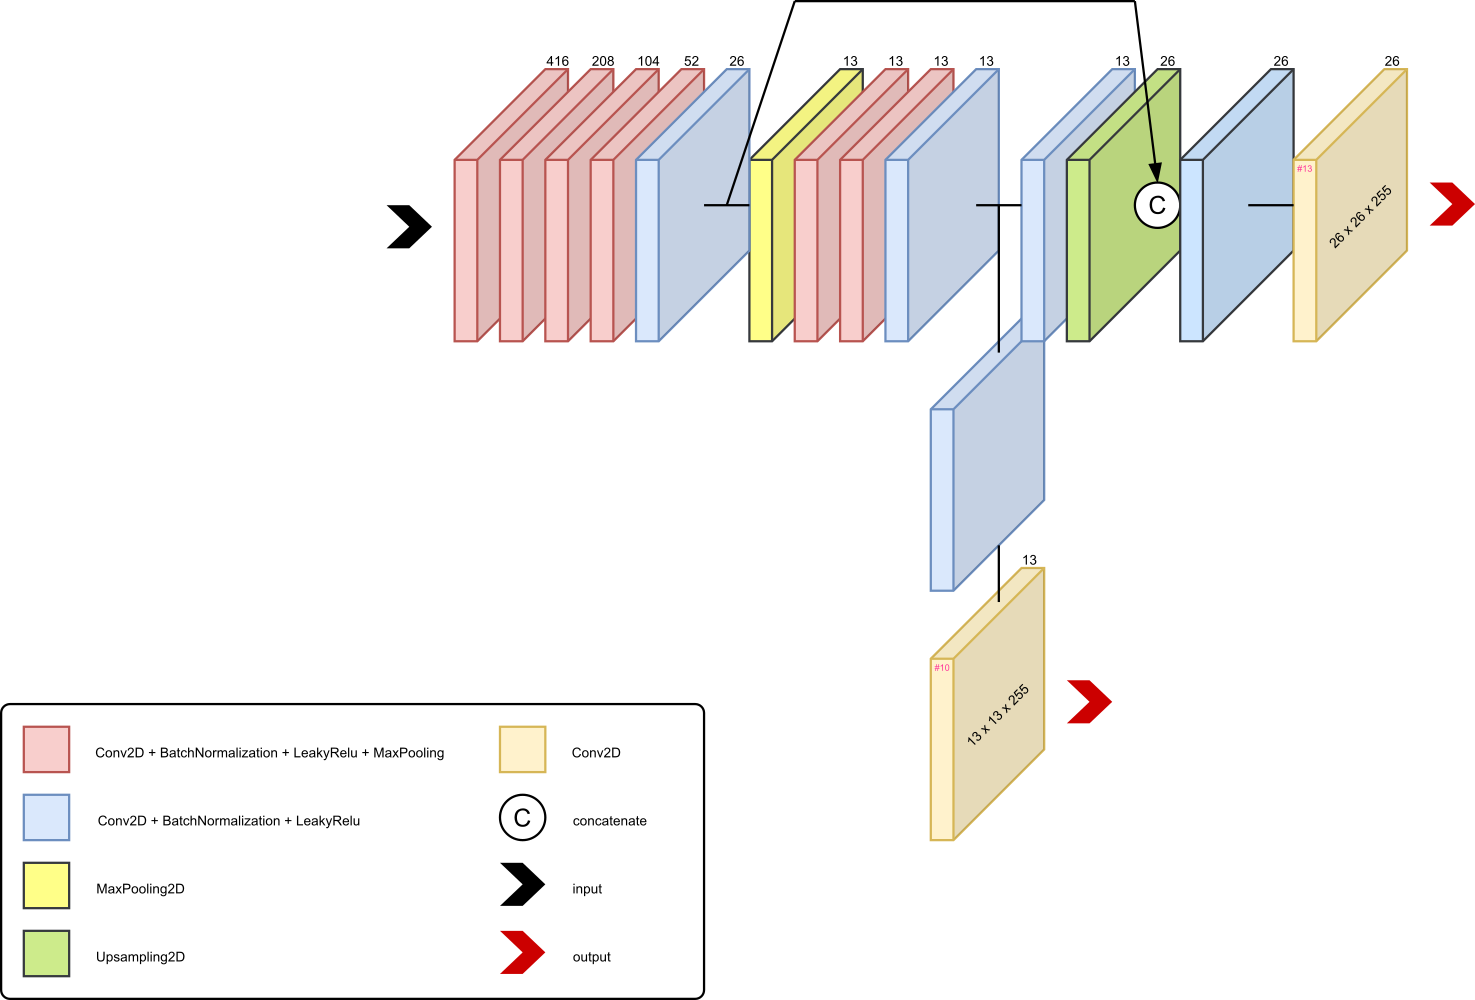
\includegraphics[width=\linewidth]{images/yolo_v3_tiny_architecture.png}
	\caption{Arquitectura de YOLO V3 Tiny de tamaño 416x416}
	\label{fig:yolov3tinyarchitecture}
\end{figure}

\subsection{Métodos de evaluación a utilizar en el proyecto}

La métrica que se ha utilizado para evaluar los modelo obtenidos es la \textit{AP} (Average Precision), que es la métrica que se utiliza en los problemas de detección de objetos.

Antes de explicar en qué consiste la métrica \textit{AP} hay que explicar una serie de conceptos en los cuales está basada: IoU (intersección sobre la unión), precisión (precision) y sensibilidad (recall).

El concepto de \textit{IoU} mide cuánto se solapan dos regiones: la predicha y la que debería ser detectada. Se calcula dividiendo la región obtenida mediante la intersección de la región predicha y la región a detectar entre la región obtenida mediante la unión de ambas regiones.

\begin{equation}
	AP = \frac{interseci\acute{o}n}{uni\acute{o}n} = \frac{
\includegraphics[width=0.2\linewidth]{images/ap_intersection.png}}{
\includegraphics[width=0.2\linewidth]{images/ap_union.png}}
	\nonumber
\end{equation}

La \textit{precisión} (precision) mide la capacidad del modelo para detectar únicamente los objetos relevantes. Se calcula como el porcentaje de predicciones positivas acertadas frente a todas las predicciones positivas predichas:

\begin{equation}
	precisi\acute{o}n = \frac{TP}{TP + FP} = \frac{TP}{todas\ las\ predicciones\ positivas}
	\nonumber
\end{equation}

La \textit{sensibilidad} (recall)  mide la capacidad del modelo para detectar todos los objetos relevantes. Se calcula como el porcentaje de predicciones positivas acertadas frente a todas las existentes:

\begin{equation}
	sensibilidad = \frac{TP}{TP + FN} = \frac{TP}{todas\ las\ regiones\ a\ detectar}
	\nonumber
\end{equation}

Tanto en el cálculo de la \textit{precisión} como en de la \textit{sensibilidad}, para determinar si una predicción es positiva, se utiliza el \textit{IoU}. Se define un umbral para el \textit{IoU} (normalmente suele ser 0.5) y si se supera dicho umbral, la predicción es considerada positiva.

La métrica \textit{AP} se calcula como el área debajo de la curva \textit{precisión-sensibilidad} (precision-recall). En el eje de las abscisas se representa la \textit{sensibilidad} (recall) y en el eje de las ordenadas se representa la \textit{precisión} (precision).

A continuación se va a mostrar un ejemplo práctico de cómo se calcula la \textit{AP}. Para este ejemplo se dispone de una serie de imágenes con un total de 4 baches a detectar. En la tabla \ref{tab:apprecisionrecalltable} se puede ver el cálculo de la \textit{precisión} y de la \textit{sensibilidad} para las predicciones obtenidas. La columna \textit{Positivo} indica si la predicción es positiva, es decir, si el valor de \textit{IoU} supera el umbral definido, que en este caso es 0.5. Las columnas \textit{TP} y \textit{FP} muestran el acumulado de sus respectivos valores.

\begin{table}[H]
	\centering
	\begin{tabular}{rrrrrr}
		\toprule
		IoU &  Positivo &  TP &  FP &  Precisión &  Sensibilidad \\
		\midrule
		0.912933 &         1 &   1 &   0 &   1.000000 &          0.25 \\
		0.711111 &         1 &   2 &   0 &   1.000000 &          0.50 \\
		0.387983 &         0 &   2 &   1 &   0.666667 &          0.50 \\
		0.387983 &         0 &   2 &   2 &   0.500000 &          0.50 \\
		0.387983 &         0 &   2 &   3 &   0.400000 &          0.50 \\
		1.000000 &         1 &   3 &   3 &   0.500000 &          0.75 \\
		0.225986 &         0 &   3 &   4 &   0.428571 &          0.75 \\
		0.225986 &         0 &   3 &   5 &   0.375000 &          0.75 \\
		1.000000 &         1 &   4 &   5 &   0.444444 &          1.00 \\
		\bottomrule
	\end{tabular}
	\caption{Cálculo de la precisión y sensibilidad para las predicciones}
	\label{tab:apprecisionrecalltable}
\end{table}

Una vez se tienen calculados los valores de \textit{precisión} y de \textit{sensibilidad} se calcula la curva \textit{precisión-sensibilidad} como se puede ver en la figura \ref{fig:apprecisionrecallcurve}. Para realizar el cálculo del área debajo de la curva se realiza un suavizado de la misma. Este suavizado consiste en establecer como valor de \textit{precisión} para un determinado valor de \textit{sensibilidad}, el valor de \textit{precisión} más alto que se encuentre a su derecha. Por ejemplo, para la \textit{sensibilidad} 0.6 se establece como valor de \textit{precisión} el valor más alto a su derecha, que en este caso es 0.5. En color naranja se puede ver la curva suavizada.

\begin{figure}[H]
	\centering
	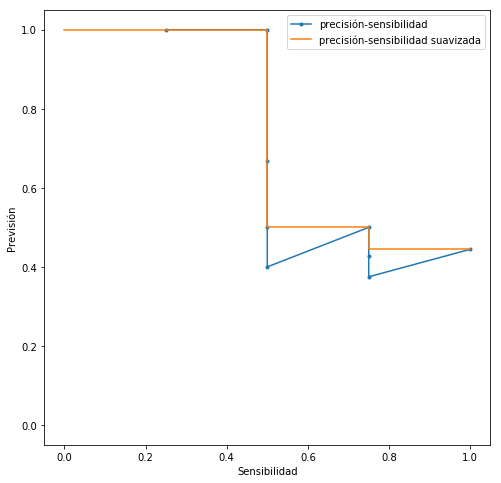
\includegraphics[width=0.7\linewidth]{images/ap_precision_recall_curve.png}
	\caption{Curva precisión-sensibilidad}
	\label{fig:apprecisionrecallcurve}
\end{figure}

Por lo que finalmente, para este ejemplo, el cálculo del \textit{AP} sería:

\begin{equation}
	AP = (0.5 - 0) \cdot 1 + (0.75 - 0.5) \cdot 0.5 + (1 - 0.75) \cdot 0.44 = 0.5 + 0.125 + 0.11 = \textbf{0.735}
	\nonumber
\end{equation} % (<6 páginas)

\newpage
\section{Implementación y evaluación de las técnicas}

% (Aquí no te pongo límite de páginas. Explícalo como quieras ya que es la parte en la que tienes que explicar el trabajo técnico que has realizado.)

\subsection{Detalles de la implementación de las técnicas de DL aplicadas}

% (Esto sería parte práctica)
% una especie de bitácora sin hablar en primera persona

\textbf{!!! TODO}

\subsection{Evaluación de las técnicas}

% (Esto sería parte práctica)

\textbf{!!! TODO} % (Aquí no te pongo límite de páginas)

\newpage
\section{Resultados}
\label{sec:resultados}

\subsection{Resultados del proyecto}

En esta sección se van a mostrar algunos ejemplos de las predicciones obtenidas con los modelos entrenados con el conjunto de datos que mejores resultados ha obtenido, es decir, con los modelos entrenados con el juego de datos denominado como \textit{filtro 100x40}. Este juego de datos está compuesto por imágenes con baches que como mínimo tienen unas dimensiones de 100x40 píxeles.

\begin{figure}[H]
	\centering
	\begin{subfigure}[h]{0.45\linewidth}
		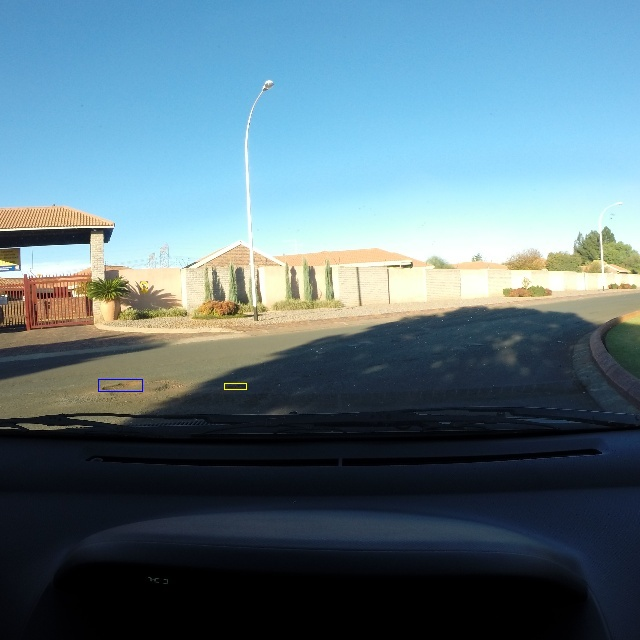
\includegraphics[width=\linewidth]{images/results_a_gt.jpg}
		\caption{Baches a detectar}
	\end{subfigure}
	\begin{subfigure}[h]{0.45\linewidth}
		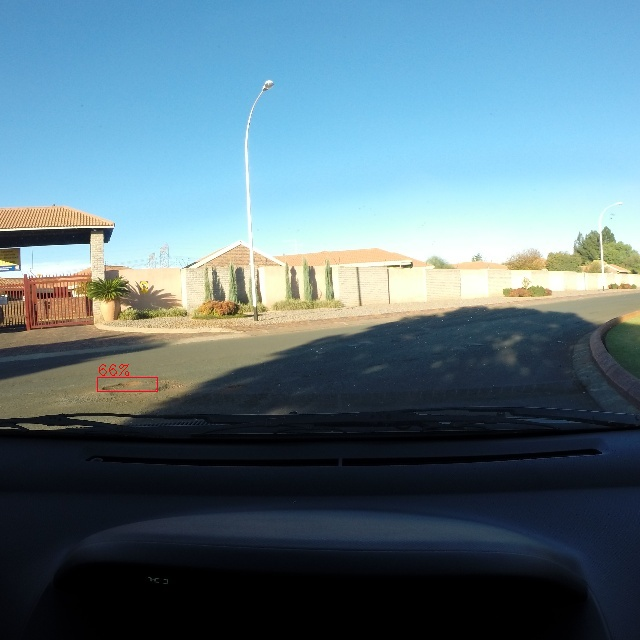
\includegraphics[width=\linewidth]{images/results_a_yolo_v3_256.jpg}
		\caption{YOLO V3 tamaño 256x256}
	\end{subfigure}
	\begin{subfigure}[h]{0.45\linewidth}
		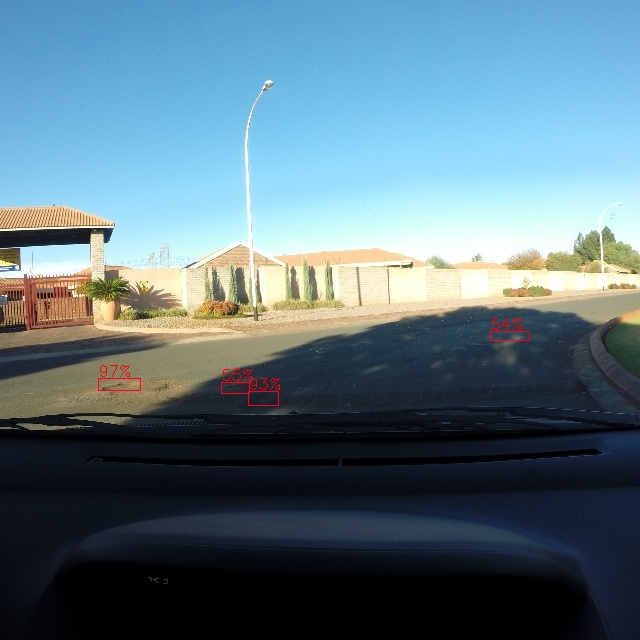
\includegraphics[width=\linewidth]{images/results_a_yolo_v3_416.jpg}
		\caption{YOLO V3 tamaño 416x416}
	\end{subfigure}
	\begin{subfigure}[h]{0.45\linewidth}
		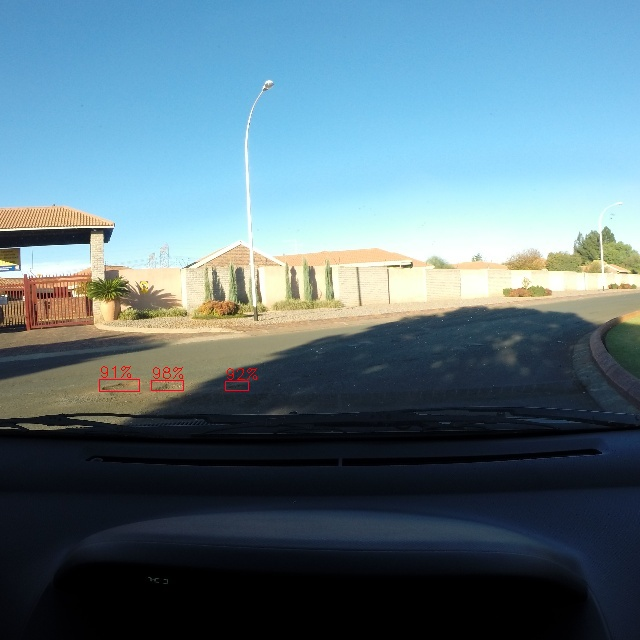
\includegraphics[width=\linewidth]{images/results_a_yolo_v3_640.jpg}
		\caption{YOLO V3 tamaño 640x640}
	\end{subfigure}
	\caption{Ejemplo de predicción con modelos YOLO V3 de distintos tamaños. Arriba a la izquierda, la imagen con los baches a detectar en azul y en amarillo los baches que fueron descartados por el filtro. En el resto de las imágenes se pueden ver las predicciones realizadas en rojo.}
	\label{fig:resultsav3}
\end{figure}

En la figura \ref{fig:resultsav3} se muestran las predicciones realizadas por los modelos YOLO V3. Se trata de una imagen en la que originalmente se han etiquetado 2 baches, uno de los cuales se ha descartado por ser demasiado pequeño. Se puede observar que existe un defecto en el etiquetado, ya que entre los dos baches etiquetados existe un tercer bache sin etiquetar. Aún habiendo filtrado los baches pequeños se puede comprobar los modelos más grandes son capaces de detectarlos. También se puede observar que el modelo de tamaño 640x640 es capaz de detectar el bache sin etiquetar.

En la figura \ref{fig:resultsav3tiny} se muestran las predicciones realizadas por los modelos YOLO V3 Tiny para la misma imagen. Únicamente el modelo de tamaño 416x416 es capaz de detectar el bache, aunque lo hace de manera poco precisa ya que la región detectada es demasiado grande y abarca también al bache sin etiquetar.

\begin{figure}[H]
	\centering
	\begin{subfigure}[h]{0.45\linewidth}
		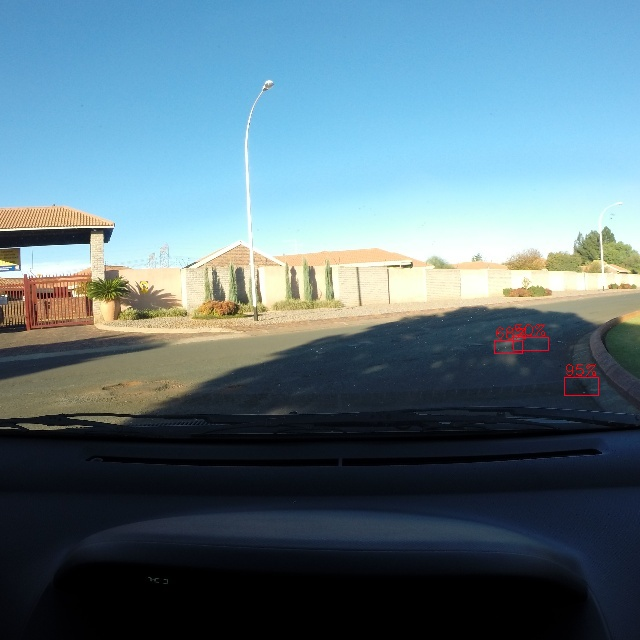
\includegraphics[width=\linewidth]{images/results_a_yolo_v3_tiny_256.jpg}
		\caption{YOLO V3 Tiny tamaño 256x256}
	\end{subfigure}
	\begin{subfigure}[h]{0.45\linewidth}
		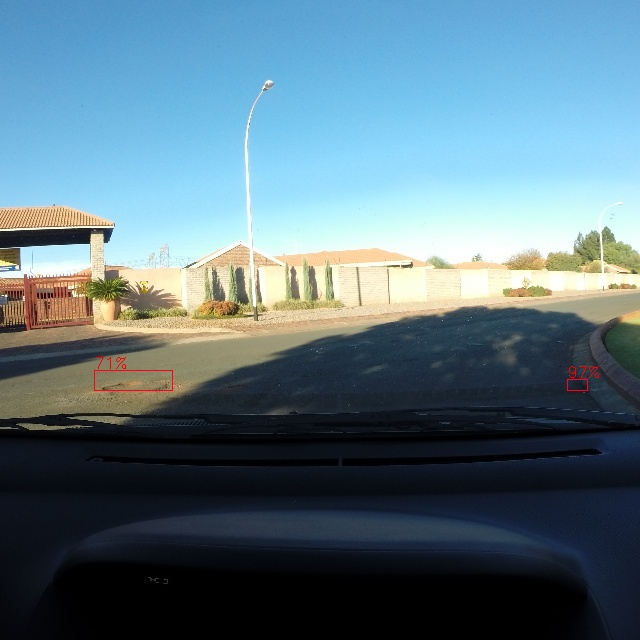
\includegraphics[width=\linewidth]{images/results_a_yolo_v3_tiny_416.jpg}
		\caption{YOLO V3 Tiny tamaño 416x416}
	\end{subfigure}
	\caption{Misma predicción que en la figura \ref{fig:resultsav3}, pero en esta ocasión con modelos YOLO V3 Tiny.}
	\label{fig:resultsav3tiny}
\end{figure}

En la figura \ref{fig:resultsbv3} se muestran más predicciones realizadas por los modelos YOLO V3. En esta ocasión se trata de una imagen en la que hay múltiples baches, de los cuales únicamente se han mantenido 2 y el resto se han descartado. En esta ocasión los 3 modelos detectan baches de forma correcta. El único modelo que detecta los baches esperados es el de tamaño 640x640. Además de detectar los baches detectados, es capaz de detectar uno de los baches que fue descartado por tamaño. Los otros dos modelos de tamaño inferior únicamente detectan uno de los baches esperados, aunque son capaces de detectar también algunos de los baches descartados.

\begin{figure}[H]
	\centering
	\begin{subfigure}[h]{0.45\linewidth}
		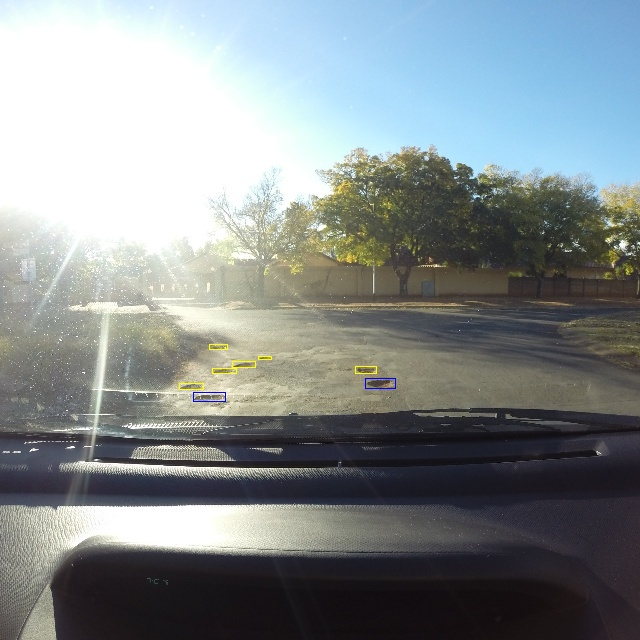
\includegraphics[width=\linewidth]{images/results_b_gt.jpg}
		\caption{Baches a detectar}
	\end{subfigure}
	\begin{subfigure}[h]{0.45\linewidth}
		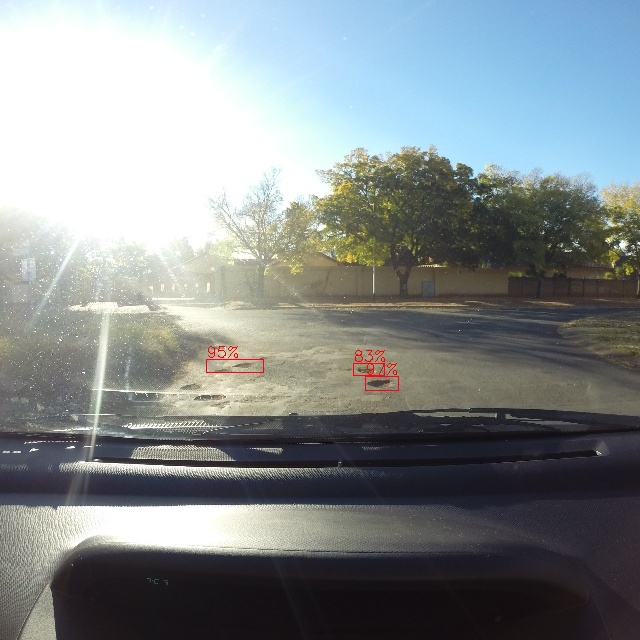
\includegraphics[width=\linewidth]{images/results_b_yolo_v3_256.jpg}
		\caption{YOLO V3 tamaño 256x256}
	\end{subfigure}
	\begin{subfigure}[h]{0.45\linewidth}
		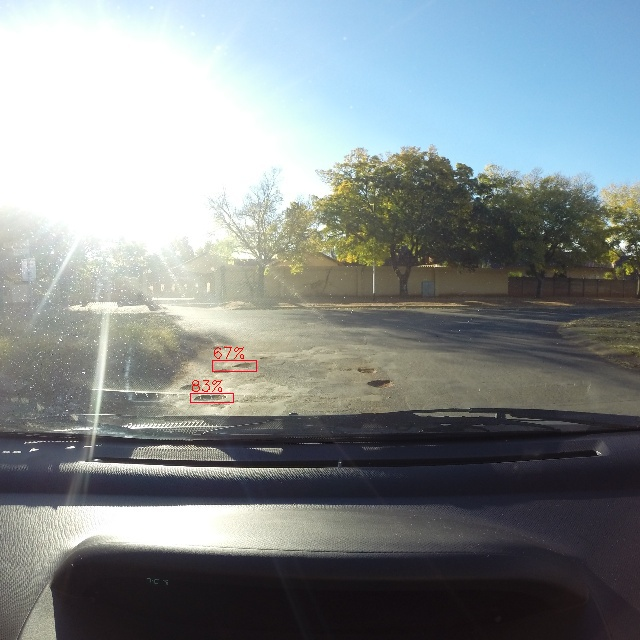
\includegraphics[width=\linewidth]{images/results_b_yolo_v3_416.jpg}
		\caption{YOLO V3 tamaño 416x416}
	\end{subfigure}
	\begin{subfigure}[h]{0.45\linewidth}
		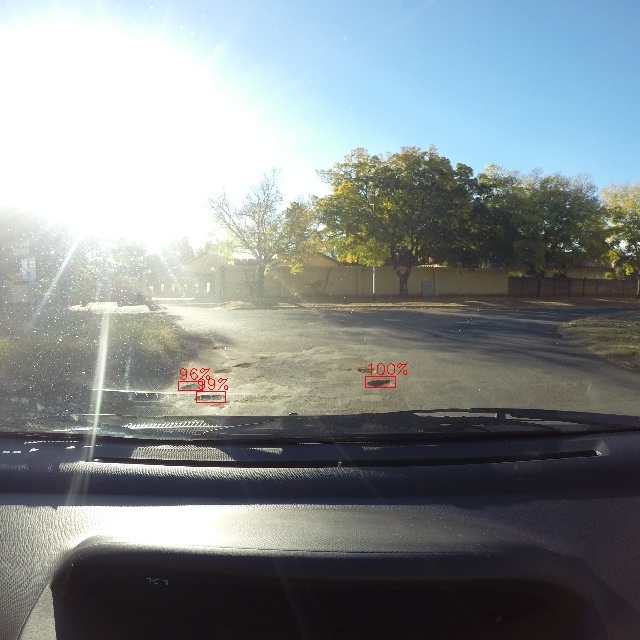
\includegraphics[width=\linewidth]{images/results_b_yolo_v3_640.jpg}
		\caption{YOLO V3 tamaño 640x640}
	\end{subfigure}
	\caption{Ejemplo de predicción con modelos YOLO V3 de distintos tamaños. Arriba a la izquierda, la imagen con los baches a detectar en azul y en amarillo los baches que fueron descartados por el filtro. En el resto de las imágenes se pueden ver las predicciones realizadas en rojo.}
	\label{fig:resultsbv3}
\end{figure}

En la figura \ref{fig:resultsbv3tiny} se muestran las predicciones realizadas por los modelos YOLO V3 Tiny para el segundo ejemplo. En esta ocasión ambos modelos son capaces de detectar baches de forma correcta. Además el modelo de tamaño 416x416 es capaz de identificar los dos baches esperados.

\begin{figure}[H]
	\centering
	\begin{subfigure}[h]{0.45\linewidth}
		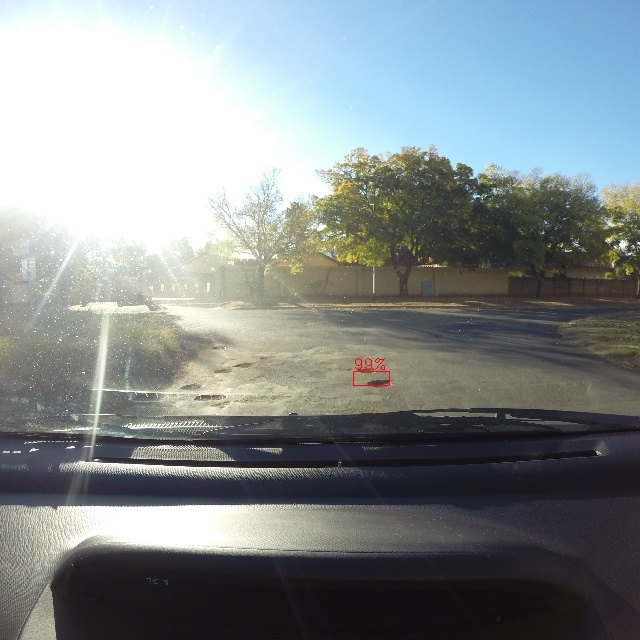
\includegraphics[width=\linewidth]{images/results_b_yolo_v3_tiny_256.jpg}
		\caption{YOLO V3 Tiny tamaño 256x256}
	\end{subfigure}
	\begin{subfigure}[h]{0.45\linewidth}
		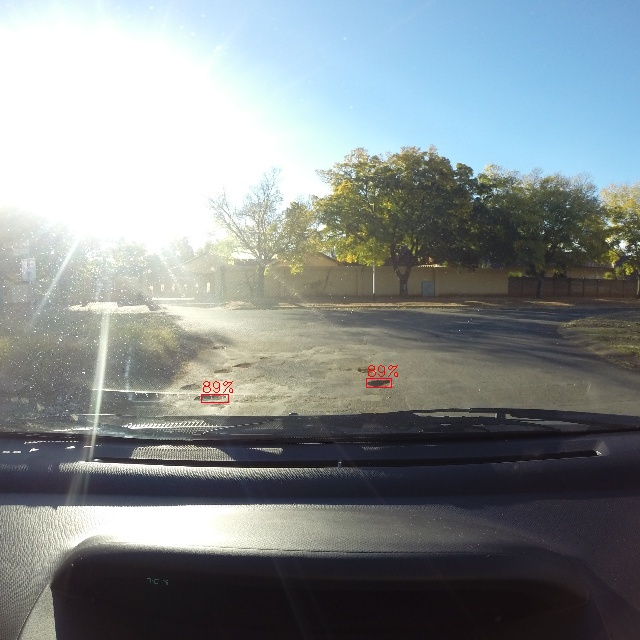
\includegraphics[width=\linewidth]{images/results_b_yolo_v3_tiny_416.jpg}
		\caption{YOLO V3 Tiny tamaño 416x416}
	\end{subfigure}
	\caption{Misma predicción que en la figura \ref{fig:resultsbv3}, pero en esta ocasión con modelos YOLO V3 Tiny.}
	\label{fig:resultsbv3tiny}
\end{figure}

En la figura \ref{fig:resultscv3} se muestra otro ejemplo de predicciones realizadas por los modelos YOLO V3. En esta ocasión también se trata de una imagen en la que hay múltiples baches, de los cuales se ha mantenido un único bache. En esta ocasión uno de los modelos, el de tamaño 416x416, es incapaz de detectar ningún bache. El modelo más pequeño, detecta uno de los baches que ha sido descartado, y además la predicción es mejor al original ya que la región predicha se ajusta más al bache. El modelo más grande ha sido capaz de detectar el bache original y además detecta otro de los baches que fue descartados.

\begin{figure}[H]
	\centering
	\begin{subfigure}[h]{0.45\linewidth}
		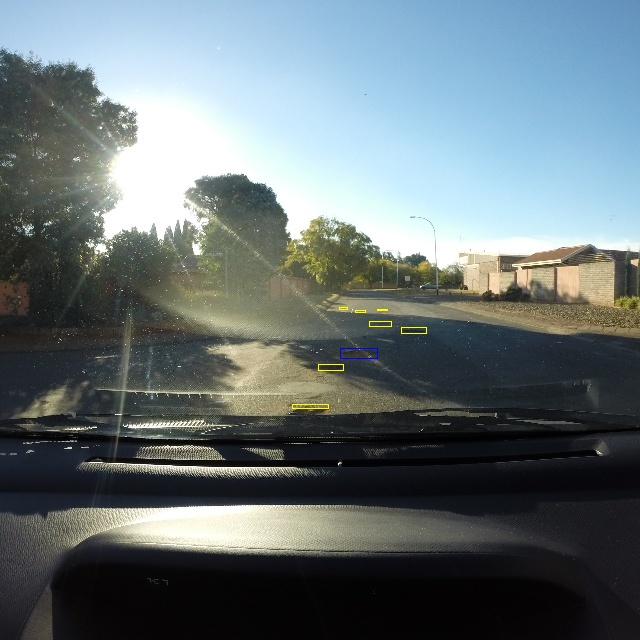
\includegraphics[width=\linewidth]{images/results_c_gt.jpg}
		\caption{Baches a detectar}
	\end{subfigure}
	\begin{subfigure}[h]{0.45\linewidth}
		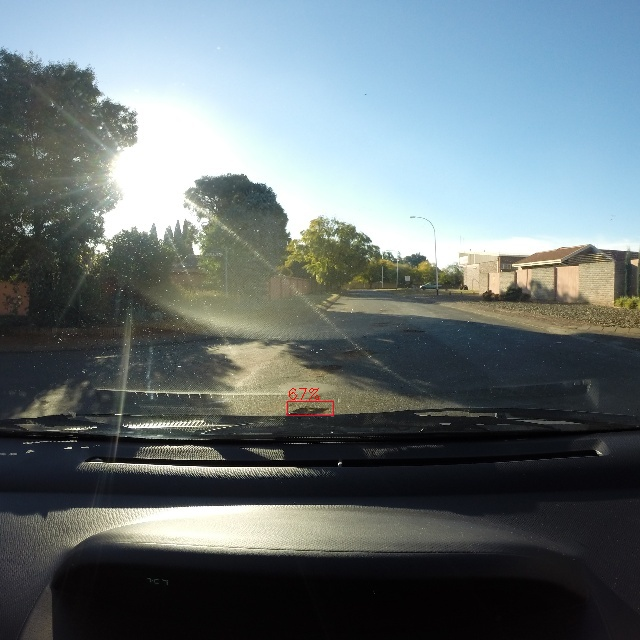
\includegraphics[width=\linewidth]{images/results_c_yolo_v3_256.jpg}
		\caption{YOLO V3 tamaño 256x256}
	\end{subfigure}
	\begin{subfigure}[h]{0.45\linewidth}
		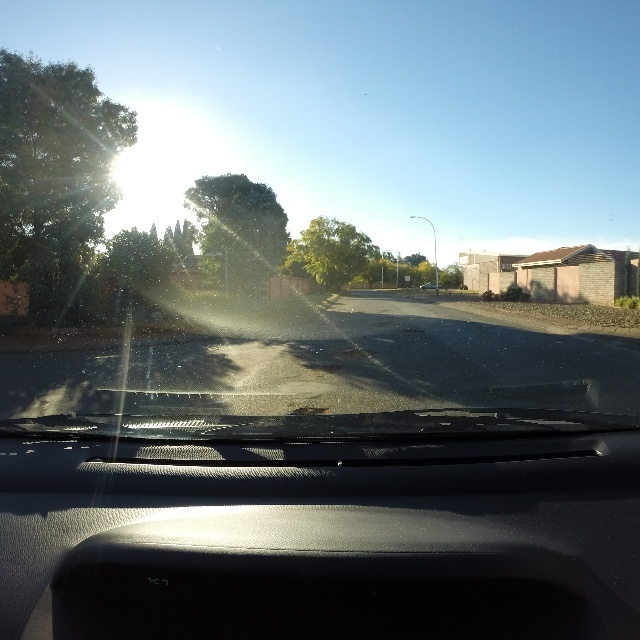
\includegraphics[width=\linewidth]{images/results_c_yolo_v3_416.jpg}
		\caption{YOLO V3 tamaño 416x416}
	\end{subfigure}
	\begin{subfigure}[h]{0.45\linewidth}
		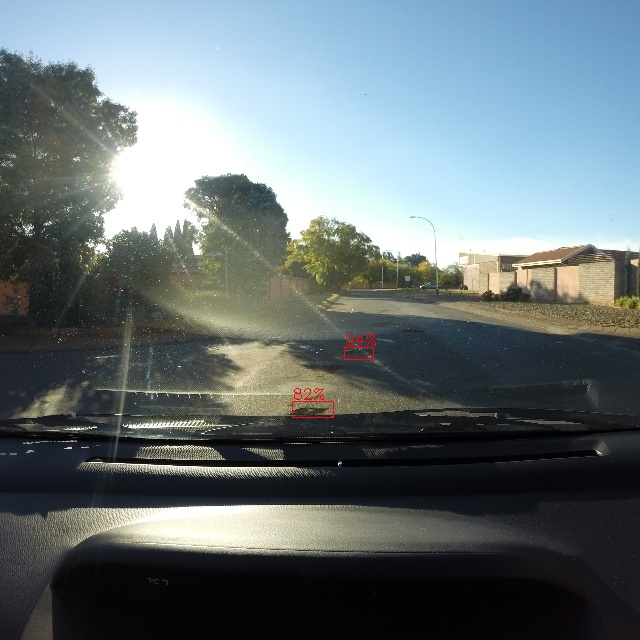
\includegraphics[width=\linewidth]{images/results_c_yolo_v3_640.jpg}
		\caption{YOLO V3 tamaño 640x640}
	\end{subfigure}
	\caption{Ejemplo de predicción con modelos YOLO V3 de distintos tamaños. Arriba a la izquierda, la imagen con los baches a detectar en azul y en amarillo los baches que fueron descartados por el filtro. En el resto de las imágenes se pueden ver las predicciones realizadas en rojo.}
	\label{fig:resultscv3}
\end{figure}

En la figura \ref{fig:resultscv3tiny} se pueden ver las predicciones realizadas por los modelos YOLO V3 Tiny para el ejemplo anterior. Sólo uno de los modelos detecta uno de los baches.

\begin{figure}[H]
	\centering
	\begin{subfigure}[h]{0.45\linewidth}
		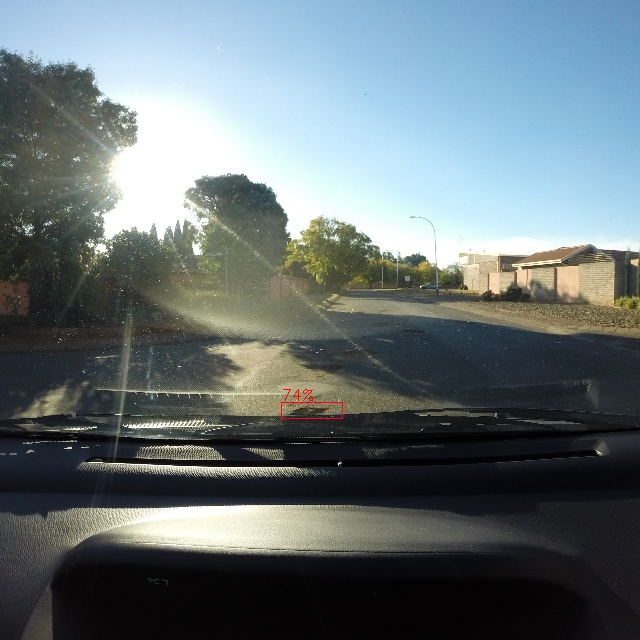
\includegraphics[width=\linewidth]{images/results_c_yolo_v3_tiny_256.jpg}
		\caption{YOLO V3 Tiny tamaño 256x256}
	\end{subfigure}
	\begin{subfigure}[h]{0.45\linewidth}
		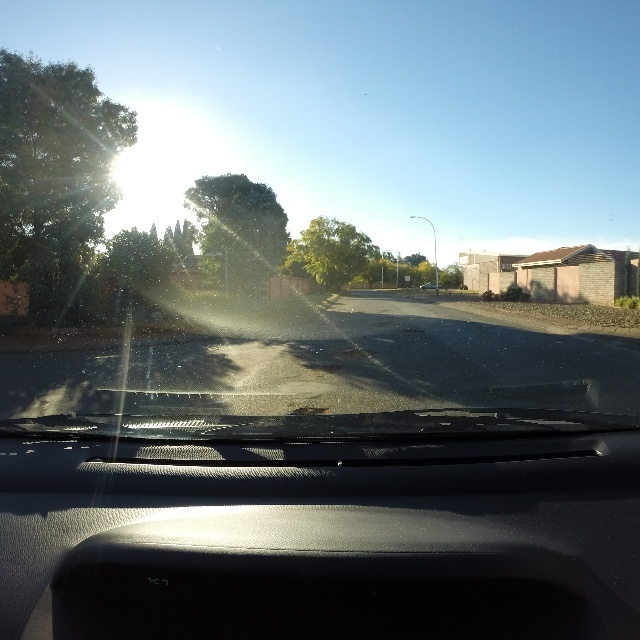
\includegraphics[width=\linewidth]{images/results_c_yolo_v3_tiny_416.jpg}
		\caption{YOLO V3 Tiny tamaño 416x416}
	\end{subfigure}
	\caption{Misma predicción que en la figura \ref{fig:resultscv3}, pero en esta ocasión con modelos YOLO V3 Tiny.}
	\label{fig:resultscv3tiny}
\end{figure}

En la figura \ref{fig:resultsdv3} se muestra un ejemplo más de predicciones realizadas por los modelos YOLO V3. En esta ocasión también se trata de una imagen en la que hay múltiples baches, de los cuales se han mantenido dos. Todos los modelos han sido capaces de detectar los baches originales, aunque no de la misma forma. Uno de los baches originales se encuentra contiguo a otro descartado. Las regiones propuestas por los dos modelos más pequeños para este bache no son muy precisas porque abarcan ambos baches. Esto no ocurre así para el modelo más grande.

\begin{figure}[H]
	\centering
	\begin{subfigure}[h]{0.45\linewidth}
		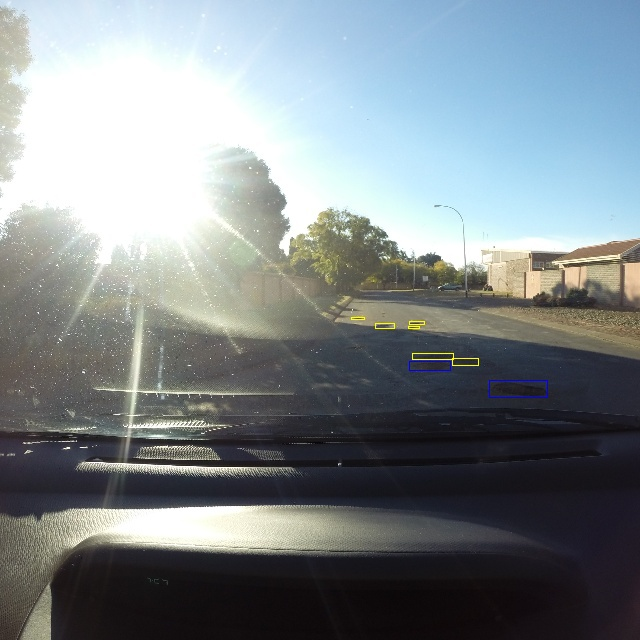
\includegraphics[width=\linewidth]{images/results_d_gt.jpg}
		\caption{Baches a detectar}
	\end{subfigure}
	\begin{subfigure}[h]{0.45\linewidth}
		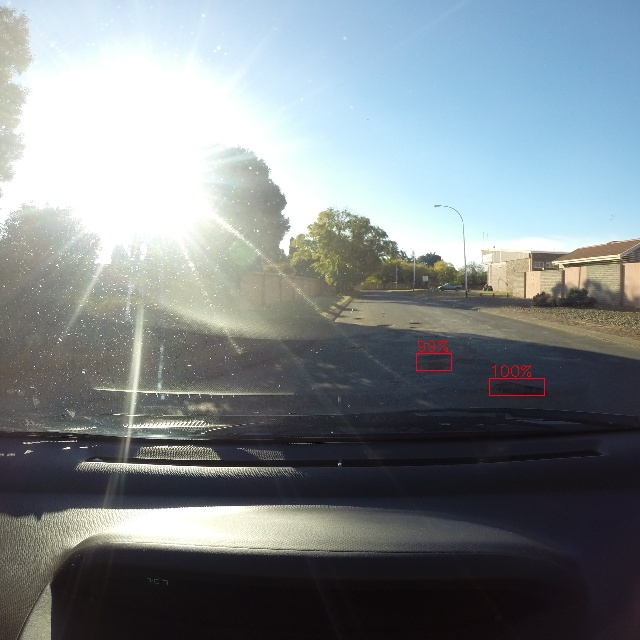
\includegraphics[width=\linewidth]{images/results_d_yolo_v3_256.jpg}
		\caption{YOLO V3 tamaño 256x256}
	\end{subfigure}
	\begin{subfigure}[h]{0.45\linewidth}
		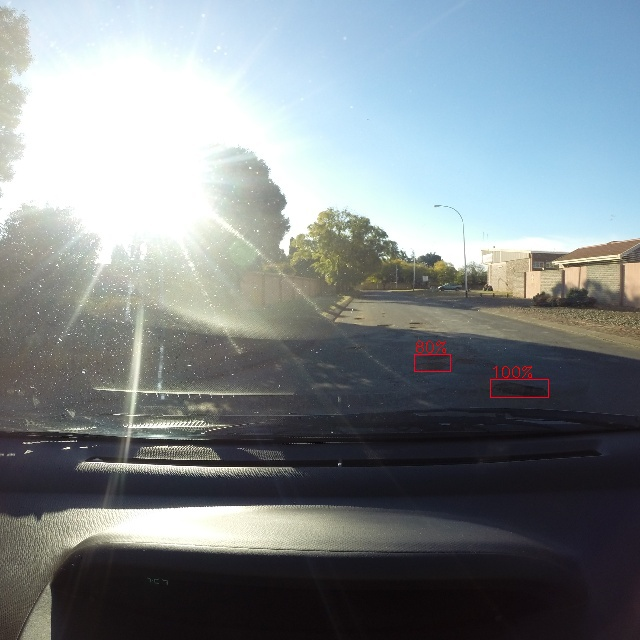
\includegraphics[width=\linewidth]{images/results_d_yolo_v3_416.jpg}
		\caption{YOLO V3 tamaño 416x416}
	\end{subfigure}
	\begin{subfigure}[h]{0.45\linewidth}
		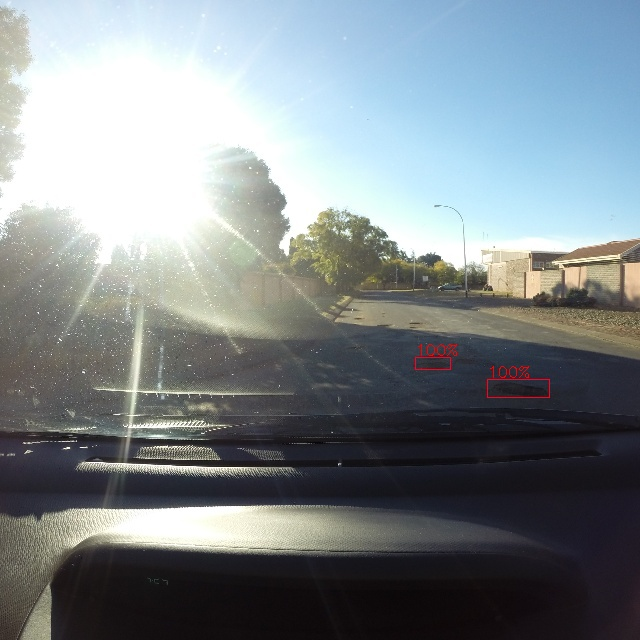
\includegraphics[width=\linewidth]{images/results_d_yolo_v3_640.jpg}
		\caption{YOLO V3 tamaño 640x640}
	\end{subfigure}
	\caption{Ejemplo de predicción con modelos YOLO V3 de distintos tamaños. Arriba a la izquierda, la imagen con los baches a detectar en azul y en amarillo los baches que fueron descartados por el filtro. En el resto de las imágenes se pueden ver las predicciones realizadas en rojo.}
	\label{fig:resultsdv3}
\end{figure}

En la figura \ref{fig:resultsdv3tiny} se pueden ver las predicciones realizadas por los modelos YOLO V3 Tiny para el ejemplo anterior. Ambos modelos detectan los baches, aunque se están haciendo predicciones adicionales que son erróneas.

\begin{figure}[H]
	\centering
	\begin{subfigure}[h]{0.45\linewidth}
		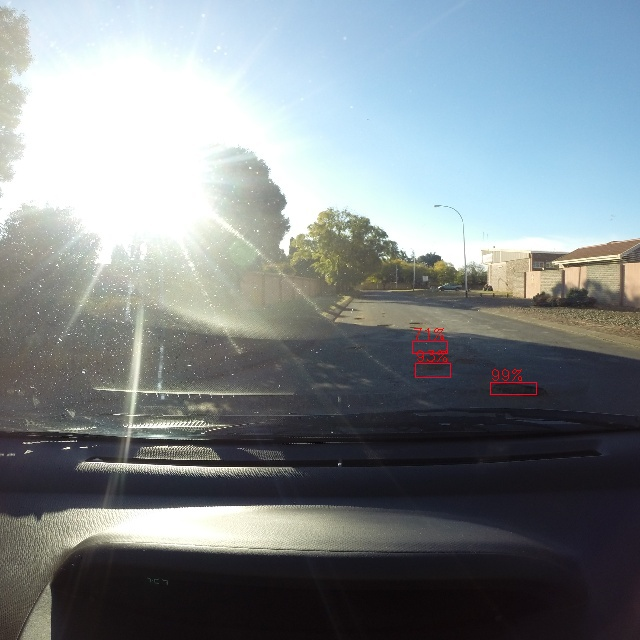
\includegraphics[width=\linewidth]{images/results_d_yolo_v3_tiny_256.jpg}
		\caption{YOLO V3 Tiny tamaño 256x256}
	\end{subfigure}
	\begin{subfigure}[h]{0.45\linewidth}
		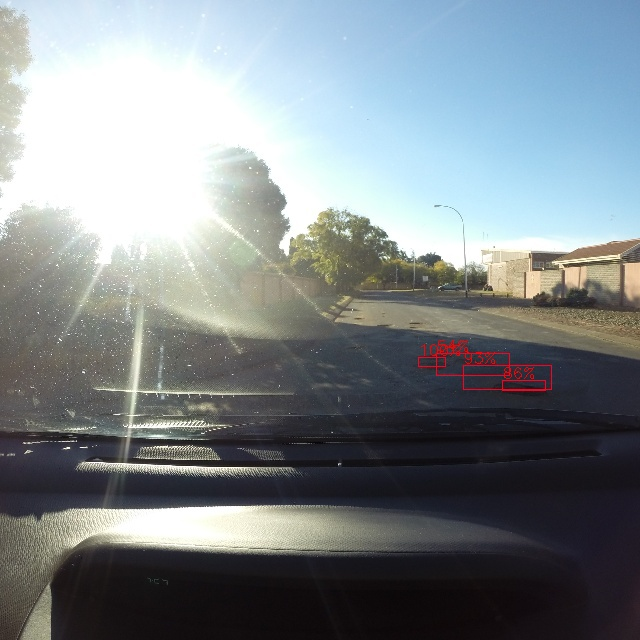
\includegraphics[width=\linewidth]{images/results_d_yolo_v3_tiny_416.jpg}
		\caption{YOLO V3 Tiny tamaño 416x416}
	\end{subfigure}
	\caption{Misma predicción que en la figura \ref{fig:resultsdv3}, pero en esta ocasión con modelos YOLO V3 Tiny.}
	\label{fig:resultsdv3tiny}
\end{figure}

En la figura \ref{fig:resultsev3} se muestra un ejemplo más de predicciones realizadas por los modelos YOLO V3. En esta ocasión también se trata de una imagen en la que hay múltiples baches, de los cuales se mantiene uno. Este ejemplo es un poco diferente a los anteriores porque este no es un caso evidente para el ojo humano, aún así, todos los modelos han sido capaces de detectar el bache original.

\begin{figure}[H]
	\centering
	\begin{subfigure}[h]{0.45\linewidth}
		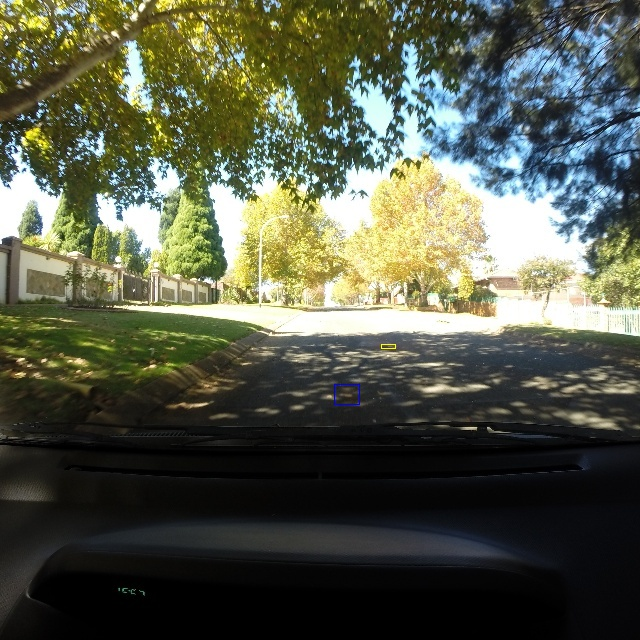
\includegraphics[width=\linewidth]{images/results_e_gt.jpg}
		\caption{Baches a detectar}
	\end{subfigure}
	\begin{subfigure}[h]{0.45\linewidth}
		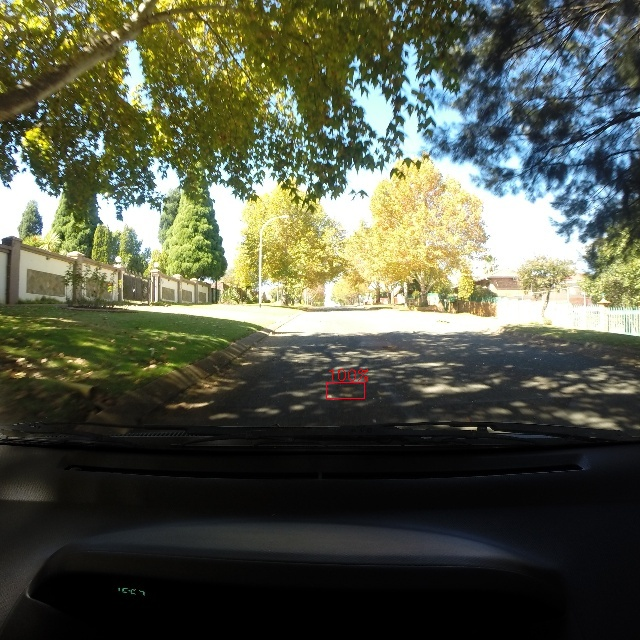
\includegraphics[width=\linewidth]{images/results_e_yolo_v3_256.jpg}
		\caption{YOLO V3 tamaño 256x256}
	\end{subfigure}
	\begin{subfigure}[h]{0.45\linewidth}
		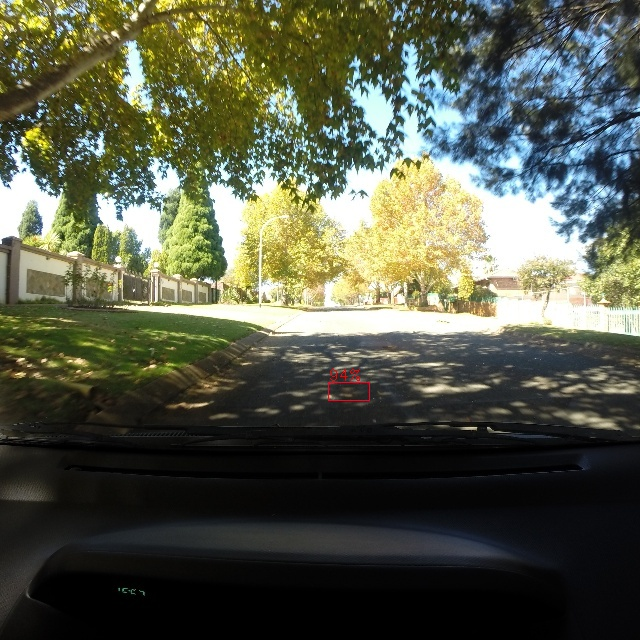
\includegraphics[width=\linewidth]{images/results_e_yolo_v3_416.jpg}
		\caption{YOLO V3 tamaño 416x416}
	\end{subfigure}
	\begin{subfigure}[h]{0.45\linewidth}
		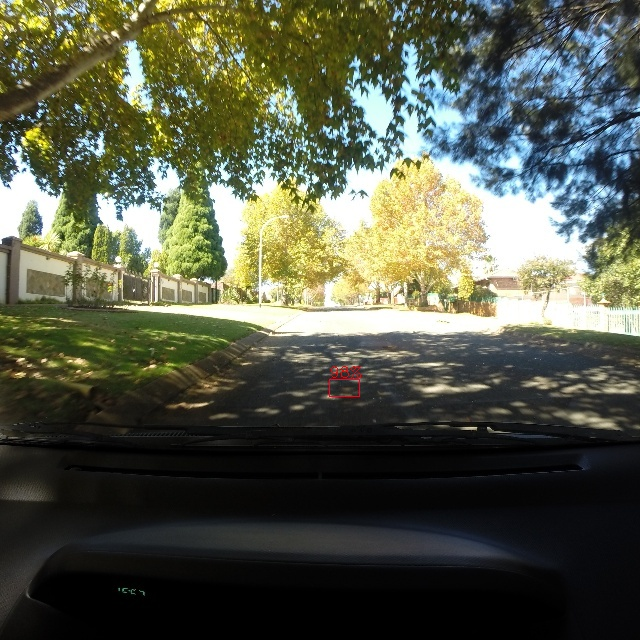
\includegraphics[width=\linewidth]{images/results_e_yolo_v3_640.jpg}
		\caption{YOLO V3 tamaño 640x640}
	\end{subfigure}
	\caption{Ejemplo de predicción con modelos YOLO V3 de distintos tamaños. Arriba a la izquierda, la imagen con los baches a detectar en azul y en amarillo los baches que fueron descartados por el filtro. En el resto de las imágenes se pueden ver las predicciones realizadas en rojo.}
	\label{fig:resultsev3}
\end{figure}

En la figura \ref{fig:resultsev3tiny} se pueden ver las predicciones realizadas por los modelos YOLO V3 Tiny para el ejemplo anterior. Sólo uno de los modelos es capaz de hacer una predicción, y además errónea.

\begin{figure}[H]
	\centering
	\begin{subfigure}[h]{0.45\linewidth}
		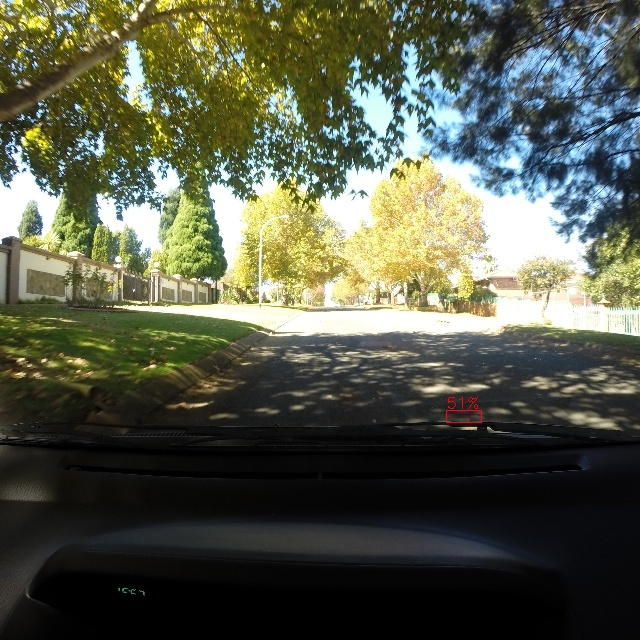
\includegraphics[width=\linewidth]{images/results_e_yolo_v3_tiny_256.jpg}
		\caption{YOLO V3 Tiny tamaño 256x256}
	\end{subfigure}
	\begin{subfigure}[h]{0.45\linewidth}
		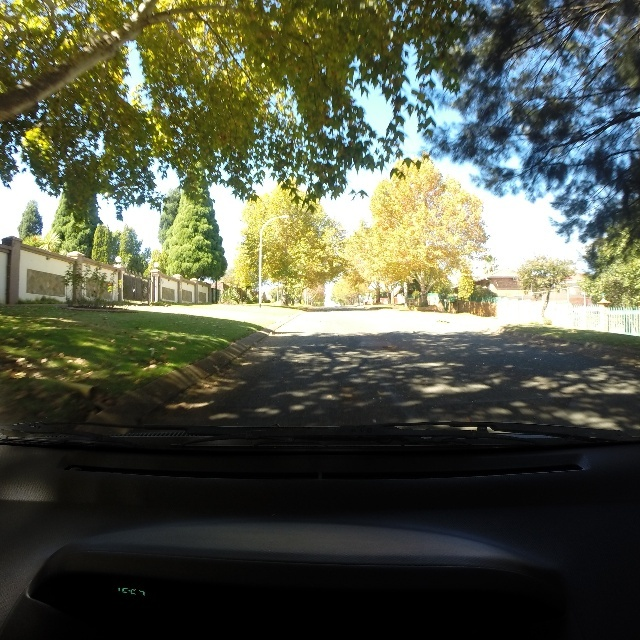
\includegraphics[width=\linewidth]{images/results_e_yolo_v3_tiny_416.jpg}
		\caption{YOLO V3 Tiny tamaño 416x416}
	\end{subfigure}
	\caption{Misma predicción que en la figura \ref{fig:resultsev3}, pero en esta ocasión con modelos YOLO V3 Tiny.}
	\label{fig:resultsev3tiny}
\end{figure}

En la figura \ref{fig:resultsfv3} se muestra un último ejemplo de predicciones realizadas por los modelos YOLO V3. En esta ocasión se trata de una imagen en la que hay un único bache. Todos los modelos tienen un comportamiento errático, además de detectar el bache, se han visto afectados por las hojas en el asfalto realizando predicciones erróneas.

\begin{figure}[H]
	\centering
	\begin{subfigure}[h]{0.45\linewidth}
		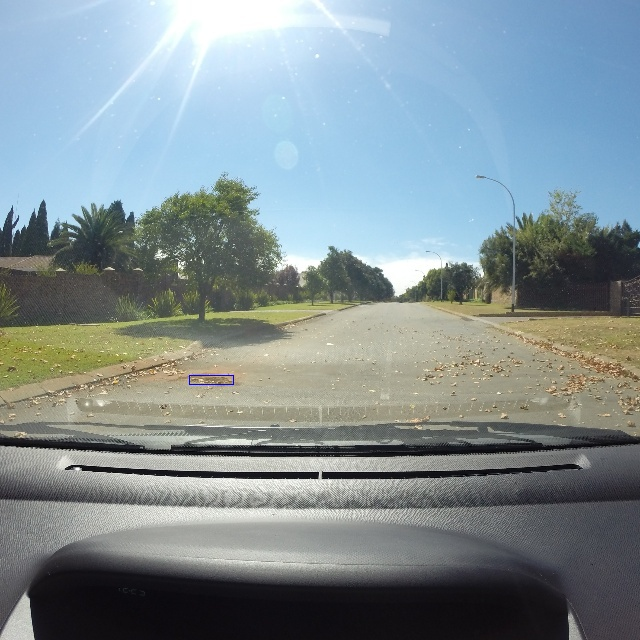
\includegraphics[width=\linewidth]{images/results_f_gt.jpg}
		\caption{Baches a detectar}
	\end{subfigure}
	\begin{subfigure}[h]{0.45\linewidth}
		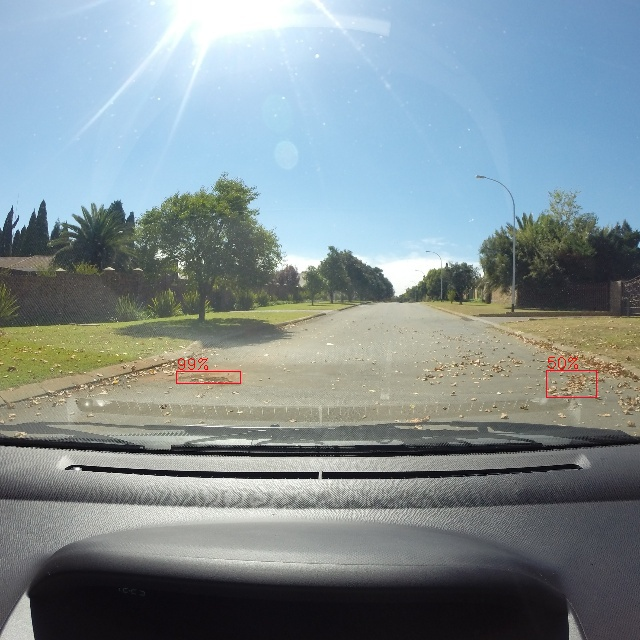
\includegraphics[width=\linewidth]{images/results_f_yolo_v3_256.jpg}
		\caption{YOLO V3 tamaño 256x256}
	\end{subfigure}
	\begin{subfigure}[h]{0.45\linewidth}
		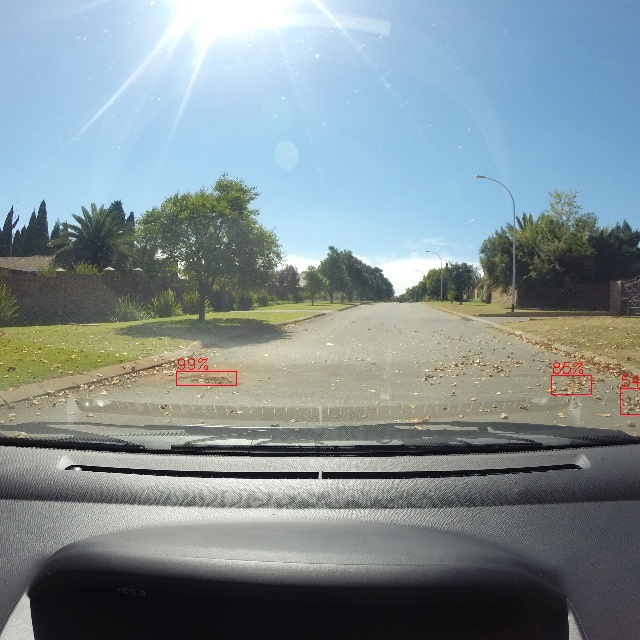
\includegraphics[width=\linewidth]{images/results_f_yolo_v3_416.jpg}
		\caption{YOLO V3 tamaño 416x416}
	\end{subfigure}
	\begin{subfigure}[h]{0.45\linewidth}
		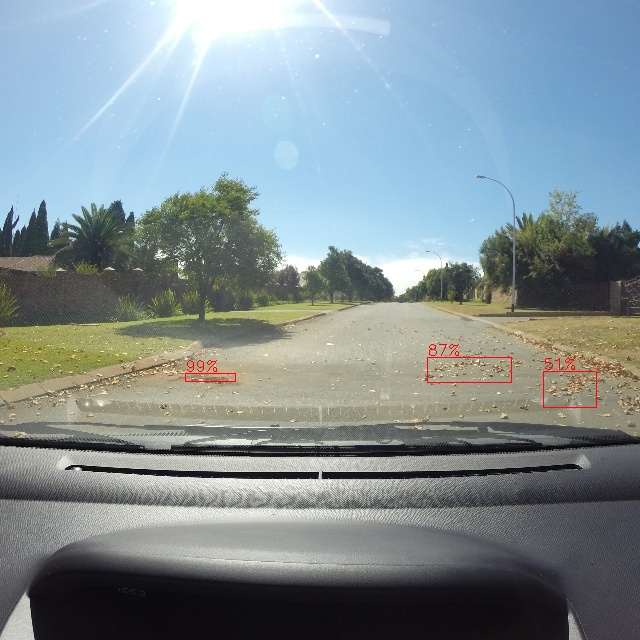
\includegraphics[width=\linewidth]{images/results_f_yolo_v3_640.jpg}
		\caption{YOLO V3 tamaño 640x640}
	\end{subfigure}
	\caption{Ejemplo de predicción con modelos YOLO V3 de distintos tamaños. Arriba a la izquierda, la imagen con los baches a detectar en azul y en amarillo los baches que fueron descartados por el filtro. En el resto de las imágenes se pueden ver las predicciones realizadas en rojo.}
	\label{fig:resultsfv3}
\end{figure}

En la figura \ref{fig:resultsfv3tiny} se pueden ver las predicciones realizadas por los modelos YOLO V3 Tiny para el ejemplo anterior. Estos modelos se han visto afectados de la misma manera por las hojas en el asfalto.

\begin{figure}[H]
	\centering
	\begin{subfigure}[h]{0.45\linewidth}
		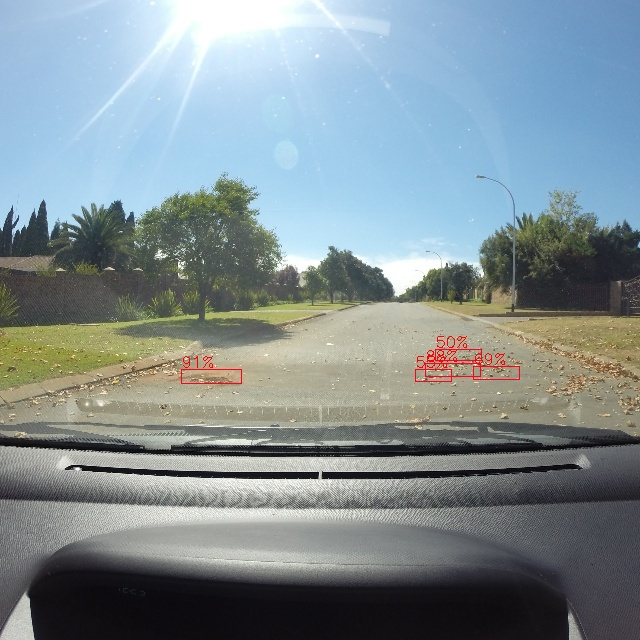
\includegraphics[width=\linewidth]{images/results_f_yolo_v3_tiny_256.jpg}
		\caption{YOLO V3 Tiny tamaño 256x256}
	\end{subfigure}
	\begin{subfigure}[h]{0.45\linewidth}
		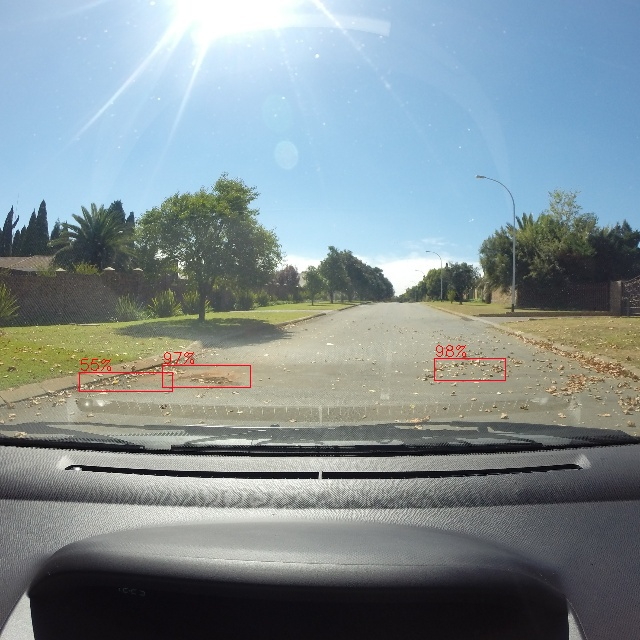
\includegraphics[width=\linewidth]{images/results_f_yolo_v3_tiny_416.jpg}
		\caption{YOLO V3 Tiny tamaño 416x416}
	\end{subfigure}
	\caption{Misma predicción que en la figura \ref{fig:resultsfv3}, pero en esta ocasión con modelos YOLO V3 Tiny.}
	\label{fig:resultsfv3tiny}
\end{figure} % (< 3 páginas)

\newpage
\section{Conclusiones}
\label{sec:conclusiones}

\subsection{Evaluación del proyecto}

% explicar lo de yolo v3 tiny después de yolo v3

Debido a las restricciones de uso del hardware se ha realizado el entrenamiento en fases, comenzando en cada fase con el modelo resultante de la fase anterior. Al finalizar cada fase se ha realizado una evaluación del modelo para ver si mejoraba con respecto a la anterior.

Se han entrenado pocas épocas, por la cantidad de tiempo que requería el entrenamiento y por la limitación de tiempo de uso del hardware. Parece que si lanzas procesos que hacen un uso intensivo del hardware, lo detectan, y a la hora de solicitar una máquina te rechazan la petición. Por lo menos, este es el comportamiento que he observado en la fase final del proyecto, en la que me costaba conseguir una máquina con GPU disponible para continuar con el entrenamiento.

Los resultados que se obtienen con TFLite desde python y desde java no son exactamente iguales, existen pequeñas diferencias a partir del 4-6 decimal, aunque no alteran demasiado las predicciones.

El rendimiento que se obtiene en el teléfono móvil me ha resultado inferior al que me esperaba. Al final con un móvil de gama media (Nokia 7 plus) se alcanzan los 5-7 FPS. También se han realizado pruebas en un móvil de gama alta (OnePlus 7P) y los resultados han sido mejores, unos 12 FPS.

{\color{red} \textbf{!!! TODO}}

\subsection{Alternativas y posibles mejoras que podrían haberse aplicado al proyecto (trabajos futuros)}

Mejorar las etiquetas de este dataset o utilizar otro dataset. Crear un dataset con carreteras de España ya que parece que los baches son diferentes, sobre todo cuando se trata de carreteras que han sido reasfaltadas y en las cuales los baches dejan al descubierto más asfalto.

Darle otro enfoque a las fotos de tal forma que estén más centradas en el asfalto y que los baches sean más grandes con respecto al tamaño de la imagen. No hace falta detectar los baches lejos, puesto que el objetivo del proyecto sería crear un inventario.

Modelo quantized para ver si se reduce el tiempo de inferencia en el dispositivo móvil

{\color{red} \textbf{!!! TODO}}

\subsection{Conclusiones personales}

{\color{red} \textbf{!!! TODO}} % (< 3  páginas)

\newpage
\nocite{*}
\printbibliography[title={Referencias}]

\end{document}